\documentclass[oneside]{book}
\usepackage{lmodern}
\usepackage{amssymb,amsmath}
\usepackage{ifxetex,ifluatex}
\usepackage{fixltx2e} % provides \textsubscript
\ifnum 0\ifxetex 1\fi\ifluatex 1\fi=0 % if pdftex
  \usepackage[T1]{fontenc}
  \usepackage[utf8]{inputenc}
\else % if luatex or xelatex
  \ifxetex
    \usepackage{mathspec}
  \else
    \usepackage{fontspec}
  \fi
  \defaultfontfeatures{Ligatures=TeX,Scale=MatchLowercase}
\fi
% use upquote if available, for straight quotes in verbatim environments
\IfFileExists{upquote.sty}{\usepackage{upquote}}{}
% use microtype if available
\IfFileExists{microtype.sty}{%
\usepackage[]{microtype}
\UseMicrotypeSet[protrusion]{basicmath} % disable protrusion for tt fonts
}{}
\PassOptionsToPackage{hyphens}{url} % url is loaded by hyperref
\usepackage[unicode=true]{hyperref}
\hypersetup{
            pdftitle={Vegetation modelling},
            pdfauthor={Hans Verbeeck, Louise Terryn, Félicien Meunier},
            pdfborder={0 0 0},
            breaklinks=true}
\urlstyle{same}  % don't use monospace font for urls
\usepackage[left=3cm,right=3cm,top=2cm,bottom=2cm]{geometry}
\usepackage{natbib}
\bibliographystyle{apalike}
\usepackage{color}
\usepackage{fancyvrb}
\newcommand{\VerbBar}{|}
\newcommand{\VERB}{\Verb[commandchars=\\\{\}]}
\DefineVerbatimEnvironment{Highlighting}{Verbatim}{commandchars=\\\{\}}
% Add ',fontsize=\small' for more characters per line
\usepackage{framed}
\definecolor{shadecolor}{RGB}{248,248,248}
\newenvironment{Shaded}{\begin{snugshade}}{\end{snugshade}}
\newcommand{\KeywordTok}[1]{\textcolor[rgb]{0.13,0.29,0.53}{\textbf{#1}}}
\newcommand{\DataTypeTok}[1]{\textcolor[rgb]{0.13,0.29,0.53}{#1}}
\newcommand{\DecValTok}[1]{\textcolor[rgb]{0.00,0.00,0.81}{#1}}
\newcommand{\BaseNTok}[1]{\textcolor[rgb]{0.00,0.00,0.81}{#1}}
\newcommand{\FloatTok}[1]{\textcolor[rgb]{0.00,0.00,0.81}{#1}}
\newcommand{\ConstantTok}[1]{\textcolor[rgb]{0.00,0.00,0.00}{#1}}
\newcommand{\CharTok}[1]{\textcolor[rgb]{0.31,0.60,0.02}{#1}}
\newcommand{\SpecialCharTok}[1]{\textcolor[rgb]{0.00,0.00,0.00}{#1}}
\newcommand{\StringTok}[1]{\textcolor[rgb]{0.31,0.60,0.02}{#1}}
\newcommand{\VerbatimStringTok}[1]{\textcolor[rgb]{0.31,0.60,0.02}{#1}}
\newcommand{\SpecialStringTok}[1]{\textcolor[rgb]{0.31,0.60,0.02}{#1}}
\newcommand{\ImportTok}[1]{#1}
\newcommand{\CommentTok}[1]{\textcolor[rgb]{0.56,0.35,0.01}{\textit{#1}}}
\newcommand{\DocumentationTok}[1]{\textcolor[rgb]{0.56,0.35,0.01}{\textbf{\textit{#1}}}}
\newcommand{\AnnotationTok}[1]{\textcolor[rgb]{0.56,0.35,0.01}{\textbf{\textit{#1}}}}
\newcommand{\CommentVarTok}[1]{\textcolor[rgb]{0.56,0.35,0.01}{\textbf{\textit{#1}}}}
\newcommand{\OtherTok}[1]{\textcolor[rgb]{0.56,0.35,0.01}{#1}}
\newcommand{\FunctionTok}[1]{\textcolor[rgb]{0.00,0.00,0.00}{#1}}
\newcommand{\VariableTok}[1]{\textcolor[rgb]{0.00,0.00,0.00}{#1}}
\newcommand{\ControlFlowTok}[1]{\textcolor[rgb]{0.13,0.29,0.53}{\textbf{#1}}}
\newcommand{\OperatorTok}[1]{\textcolor[rgb]{0.81,0.36,0.00}{\textbf{#1}}}
\newcommand{\BuiltInTok}[1]{#1}
\newcommand{\ExtensionTok}[1]{#1}
\newcommand{\PreprocessorTok}[1]{\textcolor[rgb]{0.56,0.35,0.01}{\textit{#1}}}
\newcommand{\AttributeTok}[1]{\textcolor[rgb]{0.77,0.63,0.00}{#1}}
\newcommand{\RegionMarkerTok}[1]{#1}
\newcommand{\InformationTok}[1]{\textcolor[rgb]{0.56,0.35,0.01}{\textbf{\textit{#1}}}}
\newcommand{\WarningTok}[1]{\textcolor[rgb]{0.56,0.35,0.01}{\textbf{\textit{#1}}}}
\newcommand{\AlertTok}[1]{\textcolor[rgb]{0.94,0.16,0.16}{#1}}
\newcommand{\ErrorTok}[1]{\textcolor[rgb]{0.64,0.00,0.00}{\textbf{#1}}}
\newcommand{\NormalTok}[1]{#1}
\usepackage{longtable,booktabs}
% Fix footnotes in tables (requires footnote package)
\IfFileExists{footnote.sty}{\usepackage{footnote}\makesavenoteenv{long table}}{}
\usepackage{graphicx,grffile}
\makeatletter
\def\maxwidth{\ifdim\Gin@nat@width>\linewidth\linewidth\else\Gin@nat@width\fi}
\def\maxheight{\ifdim\Gin@nat@height>\textheight\textheight\else\Gin@nat@height\fi}
\makeatother
% Scale images if necessary, so that they will not overflow the page
% margins by default, and it is still possible to overwrite the defaults
% using explicit options in \includegraphics[width, height, ...]{}
\setkeys{Gin}{width=\maxwidth,height=\maxheight,keepaspectratio}
\IfFileExists{parskip.sty}{%
\usepackage{parskip}
}{% else
\setlength{\parindent}{0pt}
\setlength{\parskip}{6pt plus 2pt minus 1pt}
}
\setlength{\emergencystretch}{3em}  % prevent overfull lines
\providecommand{\tightlist}{%
  \setlength{\itemsep}{0pt}\setlength{\parskip}{0pt}}
\setcounter{secnumdepth}{5}
% Redefines (sub)paragraphs to behave more like sections
\ifx\paragraph\undefined\else
\let\oldparagraph\paragraph
\renewcommand{\paragraph}[1]{\oldparagraph{#1}\mbox{}}
\fi
\ifx\subparagraph\undefined\else
\let\oldsubparagraph\subparagraph
\renewcommand{\subparagraph}[1]{\oldsubparagraph{#1}\mbox{}}
\fi

% set default figure placement to htbp
\makeatletter
\def\fps@figure{htbp}
\makeatother

\usepackage{booktabs}
\usepackage{fancyhdr}

\AtBeginDocument{\let\maketitle\relax} % To relax 

% Remove page number on page parts
\usepackage{etoolbox}
\patchcmd{\part}{\thispagestyle{plain}}{\thispagestyle{empty}}{}{}

% Header and font 
\usepackage{fancyhdr}
\pagestyle{fancy}
\fancyhf{} % sets both header and footer to nothing
\renewcommand{\headrulewidth}{0pt} % Remove line

\fancyhead[L,C,R]{} % Empty header
\fancyfoot[C]{\thepage} % Footer, center, page number
\fancyfoot[L,R]{} % Empty footer on left and right
\usepackage{caption}
\usepackage{booktabs}
\usepackage{longtable}
\usepackage{array}
\usepackage{multirow}
\usepackage{wrapfig}
\usepackage{float}
\usepackage{colortbl}
\usepackage{pdflscape}
\usepackage{tabu}
\usepackage{threeparttable}
\usepackage{threeparttablex}
\usepackage[normalem]{ulem}
\usepackage{makecell}

\title{Vegetation modelling}
\author{Hans Verbeeck, Louise Terryn, Félicien Meunier}
\date{2020-11-17}

\begin{document}
\maketitle

\newcommand{\plogo}{\fbox{$\mathcal{PL}$}} % Generic dummy publisher logo
\frontmatter


\begin{titlepage} % Suppresses headers and footers on the title page

	\centering % Centre everything on the title page
	
	\scshape % Use small caps for all text on the title page
	
	\vspace*{\baselineskip} % White space at the top of the page
	
	%------------------------------------------------
	%	Title
	%------------------------------------------------
	
	\vspace{12\baselineskip}
	
	\rule{\textwidth}{1.6pt}\vspace*{-\baselineskip}\vspace*{2pt} % Thick horizontal rule
	\rule{\textwidth}{0.4pt} % Thin horizontal rule
	
	\vspace{0.75\baselineskip} % Whitespace above the title
	
	{\LARGE Meteorology and ecoclimatology\\} % Title
	
	\vspace{0.75\baselineskip} % Whitespace below the title
	
	\rule{\textwidth}{0.4pt}\vspace*{-\baselineskip}\vspace{3.2pt} % Thin horizontal rule
	\rule{\textwidth}{1.6pt} % Thick horizontal rule
	
	\vspace{2\baselineskip} % Whitespace after the title block
	
	%------------------------------------------------
	%	Subtitle
	%------------------------------------------------
	
	Course XXXX % Subtitle or further description
	
	\vspace*{3\baselineskip} % Whitespace under the subtitle
	
	%------------------------------------------------
	%	Editor(s)
	%------------------------------------------------
	
	Written By
	
	\vspace{0.5\baselineskip} % Whitespace before the editors
	
	{\scshape Hans Verbeeck, Louise Terryn, Felicien Meunier \\} % Editor list
	
	\vspace{0.5\baselineskip} % Whitespace below the editor list
	
	\textit{Ghent University \\} % Editor affiliation
	
	\vfill % Whitespace between editor names and publisher logo
	
	%------------------------------------------------
	%	Publisher
	%------------------------------------------------
	
	%\plogo % Publisher logo
	
	
\includegraphics[width = 50mm]{figures/UGhent2.png}
	
	\vspace{0.3\baselineskip} % Whitespace under the publisher logo
	
	2020 % Publication year
	
	%{\large publisher} % Publisher

\end{titlepage}

{
\setcounter{tocdepth}{1}
\tableofcontents
}
\chapter*{Prerequisites}\label{prerequisites}
\addcontentsline{toc}{chapter}{Prerequisites}

\mainmatter

\part{Basic weather
elements}\label{part-basic-weather-elements}

\chapter{Introduction, Energy and Light}\label{intro}

\chaptermark{Intro}

\section{The earth's atmosphere}\label{the-earths-atmosphere}

The atmosphere and changes in the atmosphere are central in this course.

\subsection{The earth' spheres}\label{the-earth-spheres}

The \textbf{atmosphere} is the air above the earth surface (for several
km) which interacts with all the other spheres (pedosphere -- soil,
hydrosphere -- water, cryosphere -- ice on land, anthroposhere -- part
of the earth controlled by humans and biosphere -- biotic part of the
earth).

We will talk about the atmosphere and its interaction with the biosphere
(last part of this course) but also its interaction with the
hydrosphere, pedosphere and cryosphere.

Links between the different spheres are made though fluxes of energy,
water, gases (e.g.~CO2) and the biogeochemical cycles.

\subsection{The atmosphere's
composition}\label{the-atmospheres-composition}

The atmosphere/air is gas mixture of almost 80\% N2 and more than 20\%
O2. There are also some noble gases which, together with N2 and O2, are
present at constant concentrations in the atmosphere (no mather where on
eath you take an air sample). That's why they are called
\textbf{permanent gases} in the atmosphere.

In the contrary, the \textbf{variable gases} are present in really low
concentrations (\textless{} 0.1 volume percentage except for H2O vapor
which can vary considerably between 0 and 4 volume percentages). The
other variable gases, which depend on the location on earth and time of
the day, have variable concentrations. These are some \textbf{greenhouse
gases} such as H2O, CO2, CH4, N2O and O3. It is important to know that
greenhouse gases such as CO2 are present in very low concentrations (4
ppm \textless{} 1\%) but nevertheless have a very large impact on
radiation balance of the earth and thus climate change. We can also find
\textbf{aerosols} suspended in the air and CFKs which are responsible
for the hole in the ozon layer (again, low concentrations but very
reactive).

\begin{center}
\captionof{table}{Example of Table}
\label{table:example}
\begin{tabular}{|l|l|l|l|}
\hline
Johnson Family & Transformation & Parameter Conditions & X Condition \\ \hline
$S_B$ & $Z=\gamma + \eta ln(\frac {X - \epsilon} {\lambda + \epsilon - X})$ & $\eta, \lambda >0, -\infty < \gamma, \epsilon < \infty$ & $\epsilon < X < \epsilon + \lambda$ \\ \hline
$S_L$ & $Z=\gamma + \eta ln(X - \epsilon)$ & $\eta >0, -\infty < \gamma, \epsilon < \infty$ & $X > \epsilon$ \\ \hline
$S_U$ & $Z=\gamma + \eta \sinh^{-1}(\frac {X - \epsilon} {\lambda})$ & $\eta, \lambda >0, -\infty < \gamma, \epsilon < \infty$ & $-\infty < X < \infty$ \\ \hline
\end{tabular}
\end{center}

We can easily refer to Table \ref{table:example}.

Very important for weather is \textbf{water} in the atmosphere. It is
the gas in the atmosphere which is present at the most variable
concentrations. It is continuously present in the atmosphere in three
phases: as a gas (water vapour), solid particles (ice -- high white
clouds) and liquid particles (water droplets -- lower gray clouds). But
it is also an important greenhouse gas (in abundance the most important
greenhouse gas but it has not shown the recent exponential increasing
trend like CO2 and CH4). But most importantly, H2O is responsible for a
very large part of the energy transfer on the planet through phase
transitions (latent heat). Evaporation of water consumes a lot of energy
while condensation of water releases a lot of energy.

\begin{figure}

{\centering 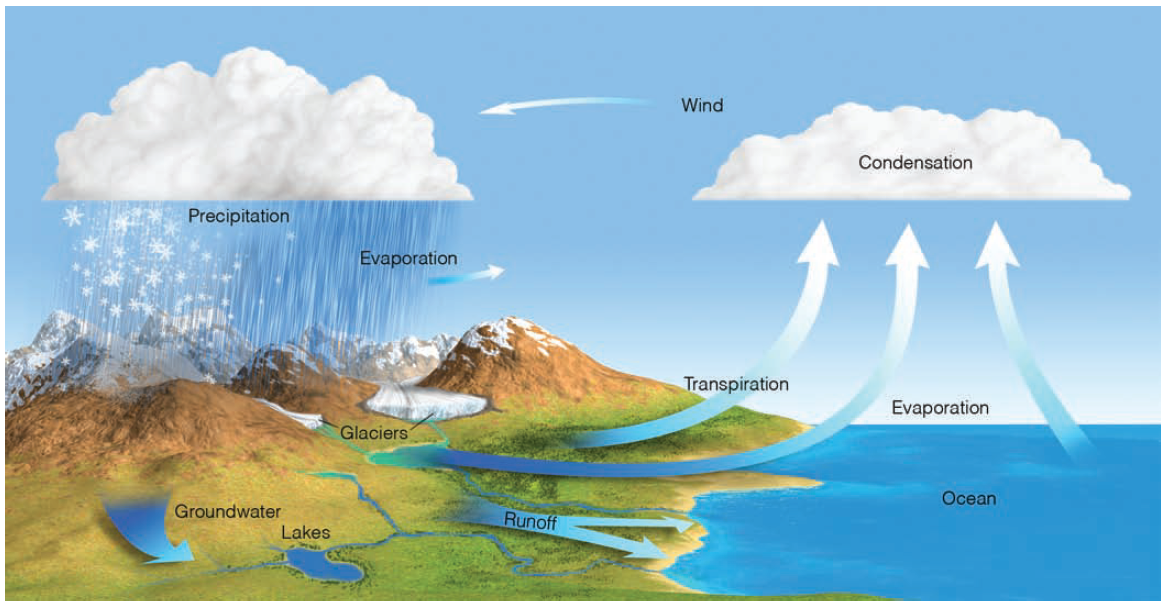
\includegraphics[width=0.8\linewidth]{figures/Figure1.1} 

}

\caption{Here is the first figure}\label{fig:intro}
\end{figure}

We can easily refer to Figure \ref{fig:intro}.

\textbf{Aerosols} are all tiny solid and liquid suspended particles in
the atmosphere which play a very important role as condensation nuclei
for cloud formation but also have an impact on radiation balance. They
can originate from anthropogenic (e.g.~industry) sources and natural
sources (e.g.~volcanic eruptions). They cause the so-called global
dimming effect. Generally, they are present in low concentrations but
these concentrations vary strongly in space and time depending on
different individual events or trends such as volcanic eruptions or
industrial activities (the latter is cause cleaner air in Europe and
more aerosols over China over the past decade).

\subsection{The atmosphere's layers}\label{the-atmospheres-layers}

Because of gravity almost all air particles are in the first km above
the earth surface. The air becomes very thin very fast. The \textbf{air
density} will decrease exponentially with height. The \textbf{air
pressure} will decrease exponentially because air pressure is the weight
of the air above it. If you are on top of the mount Everest (5.5 km
high) you are above 50\% of the air molecules. In this way we can look
at the atmosphere vertically.

However, in meteorology we mostly look at \textbf{the vertical
temperature profile}. Based on this profile the atmosphere is divided in
layers. One of the only ways to measure a vertical temperature profile
is to use a radiosonde (i.e.~weather balloon). Typically, the
temperature declines when the balloon goes higher till it reaches -50°C
at an altitude of around 10 km (airplanes fly at this height). The
temperature declines in this first layer (the \textbf{troposphere})
because the sun heats the surface, so the further from the surface the
colder it gets. The altitude where the temperature eventually stops
decreasing is called the \textbf{tropopause}. Above the tropopause there
is a \textbf{permanent temperature inversion} where the temperature will
increase with height, which is called the \textbf{stratosphere}. The
inversion is caused by the ozone layer, where ozone captures
UV-radiation of the sun, heating up the layer from the top to the
bottom. The stratosphere is a very stable layer with cold air the bottom
and warm air at the top (no turbulence, no transfer between layers --
lid on the troposphere, see chapter on atmospheric stability).
Troposphere is most important for us because this is where the weather
is. Everything we will discuss in this course are variations in the
troposphere. You don't have any cloud formation above the tropopause.
The stratosphere/inversion reaches till 50 km high where there is again
a stabilisation and the temperature will decrease with the height again
(\textbf{mesosphere}). Eventually we reach the \textbf{thermosphere}
where the temperature increases very quickly because molecules will
react very strongly with incoming solar radiation, and solar winds.
Dependent on the solar activity the temperature curve will look
differently (there is no buffer effect from the stratosphere here).

\textbf{Homosphere} is the lower part of the atmosphere where the
chemical composition is very constant (except ozone in ozone layer)
while in the \textbf{heterosphere} is very variable because of the
interaction with solar radiation.

10 km is the average \textbf{thickness of the troposphere}. Because of
the earth rotation the height of the tropopause is highest at the
equator (18 km) and lowest at the poles. This thickness also varies with
the seasons, in the summer (in the NH) there is an expansion of the
lower layer because there is more warming of the earth surface.
Therefore, the highest clouds found in Belgium are at around 10 km high
while in the tropics this will be almost double the height (till 18 km
high) and at the poles only 6 or 7 km high.

\section{Meteorology and
ecoclimatology}\label{meteorology-and-ecoclimatology}

\subsection{Difference bteween weather and
climate}\label{difference-bteween-weather-and-climate}

What is the difference between weather \& climate? Both terms are
pointing at the condition of the atmosphere, the difference lies in the
temporal perspective. \textbf{Weather} is about the short term, the
variation in the atmosphere from day to day, within days.
\textbf{Climate} is average weather (e.g. ``what is the average
temperature in September in Belgium'', ``How will this climate vary from
month to month, over the years''). Climate change is a directional
change of the average weather (e.g. ``Is our climate becoming on average
warmer?'') within timescales of decades, centuries.

If the figure below presents the probability function of temperature (or
wind speed or air humidity), then in meteorology we want to know where
we are on this curve next Tuesday for example. We want to predict or
understand why it was 25 °C yesterday and will be 15°C next Tuesday.
Climatology is what is the shape of this curve for our city, where is
the average for our city and how do the tails look for our city. If we
study climate change, then we want to know if the curve will shift, will
the shape change, will the average T be higher in our city, will the
chance to have extreme temperatures change in time? So, there is a
difference in perspective. Weather models want to predict where exactly
we are on this curve, while climate models want to predict how this full
curve will look at the end of the century, and not where we will be on
the curve on the 25 of October 2098.

\subsection{History of meteorology}\label{history-of-meteorology}

\textbf{Aristotle} was a philosopher but also the first meteorologist
who wrote a \textbf{descriptive book} (Meteorologica -- ``everything
that happens in the air'') about clouds but also about falling stars and
celestial bodies. The \textbf{next step} happened more than one thousand
years later with the invention of \textbf{measuring equipment}. Galilei
was the first person who made an instrument to measure the temperature,
the thermoscope (bubbles that rise or descend in liquids depending on
the temperature). Several decades later the barometer was invented. This
evolved till we had a set of instruments to measure weather variables
and we could start to continuously measure weather (first observations
in Ukkel in 1833). Then the first \textbf{computers} evolved to super
computers and were used quite rapidly for weather predictions and
climate modelling. After the second world war the first \textbf{radars}
were used for cloud observation and \textbf{weather satellites} were
launched. Today, ground observations are still key and are combined with
remote sensing and simulation models. What we see in weather reports is
based on the combination of these different components (e.g.~weather
stations, remote sensing, climate models). Finality of the part
meteorology in this course is reading and interpreting weather maps that
synthesize al key weather elements.

\subsection{Weather and climate in our daily
lives}\label{weather-and-climate-in-our-daily-lives}

Weather and climate are very important and determine a lot of aspects in
our lives (e.g.~agriculture, forestry, environmental issues, housing,
economy, clothing) especially extreme events as well as day to day
weather.

\subsection{Ecoclimatology}\label{ecoclimatology}

\textbf{Ecoclimatology} is an interdisciplinary science which links
ecology and climatology. It is about the link between ecosystems and the
climate, between the biosphere and the atmosphere and especially it is
about the interactions. These interactions are determined by fluxes of
energy, water and chemical elements which are exchanged between the
vegetation on the earth surface and the atmosphere.

In the ecoclimatology part of the course, we are going to talk about
biogeography, how does the climate determine which vegetation occurs on
certain places on the planet, but also about the impact of climate
variations on crops, plants, natural ecosystems and what are the
feedbacks (how do ecosystems affect the climate in their term). We will
also discuss and use vegetation models, which are important tools to
study these interactions.

\subsection{History of Ecoclimatology}\label{history-of-ecoclimatology}

\textbf{Ecoclimatology} is a younger and less developed scientific
branch which started with Theoprasthus (student of Aristotle) who wrote
a descriptive, observational book about plants and where they were
found, linked with weather patterns of that place. In the 1800s (when
measurements were possible), Alexander \textbf{von Humboldt} was the
first one who really made the link between climate and the presence of
certain plants. Later, others continued his work (e.g.~vegetation zones,
Köppen classification) and now there is also a lot of modelling.

\subsection{Biogeoscience}\label{biogeoscience}

\textbf{Biogeoscience} is closely related to ecoclimatology and is
situated on the intersection of the different spheres and studies
interactions between the different spheres. A lot of the current
environmental issues/problems have to be studied within the
biogeosciences, especially when we want to look at the anthropogenic
impact.

A good example of the role of vegetation in land-atmopshere interactions
is the given by forests. Forest provide ecosystem services, but these
are dependent on the type of forest (e.g.~a tropical rainforest versus a
boreal forest will affect the climate in different ways). For example,
the impact on the albedo (reflectivity earth surface) will be greater
when a boreal forest grows than the contribution of a tropical forest.
In the contrary, the evaporation and carbon storage of one hectare of
tropical forest will be greater than one hectare of boreal forest ((-)
cooling effect (+) warming effect).

\subsection{Key land-atmosphere
interactions}\label{key-land-atmosphere-interactions}

Interaction between land and climate has an influence on a lot of
biophysical processes. The reflectivity (\textbf{albedo}) of the earth
surface will influence the energy balance. The \textbf{roughness} of the
earth surface is determined by the type of vegetation, causing different
wind patterns and turbulence, which in its turn impacts the \textbf{heat
and gas exchange}. The physiology of the stomata of plants will have an
influence on \textbf{water exchange}. Soil moisture will also have an
impact. The \textbf{carbon cycle} has an impact on the CO2 in the
atmosphere and will depend on the type of vegetation. \textbf{Nitrogen
exchange} (N-deposition from industry or N2O as greenhouse gas from
soils) will be different in an agricultural area compared to a forest.
\textbf{Aerosols} will determine the solar radiation a forest gets which
has an impact on photosynthesis and the carbon balance. Forests will
also emit \textbf{volatile organic carbons} (e.g.~isoprene a lot in
tropical forests) which are precursors of aerosols, so forests have an
impact on the amount of aerosols in the atmosphere (also when a forest
burns this brings a lot of particles in the air). Ecoclimatology studies
many of these elements.

\section{Energy, temperature and
heat}\label{energy-temperature-and-heat}

\subsection{Definitions}\label{definitions}

\textbf{Energy} is defined as the capacity to do work. Potential
(static) and kinetic energy (dynamic) are types of energy. Energy can
take on different forms. \textbf{Temperature} is a measure for kinetic
energy (e.g.~air temperature is the kinetic energy of the air molecules
in our atmosphere). Therefore, making an energy balance is essential to
understand the climate. \textbf{Heat} is the exchange, transfer of
energy from one medium to another, it is a flux of energy.

\subsection{Temperature}\label{temperature}

Temperature is a \textbf{measure for kinetic energy} (e.g.~how much will
the molecules collide with each other and against the edges of the
volume it is confined in). Temperature is measured in ° Celsius,
Fahrenheit, Kelvin (most scientific scale). The average temperature on
earth is typically 15 °C, but weather stations typically measure
variations between -30 °C up to 40 °C.

\subsection{Specific heat}\label{specific-heat}

Different media which exist in natural systems can have very different
specific heats expressed as J per kg per °C, it is the amount of energy
needed to increase the temperature of 1 kg of a substance with 1 °C
(e.g.~a rock or sand will heat up faster than ice or wet soil -- see
table x). Water needs a very high amount of energy to heat up 1 °C (you
need four times more energy to heat up a kg of water than a kg of air).
Ice needs less energy than liquid water which is important for the
climate system (e.g.~oceans heat up slower than land and humid areas
have a large buffering capacity). This is also why there is so much heat
transfer involved with evaporation and condensation of water (latent
heat).

\subsection{Latent and sensible heat}\label{latent-and-sensible-heat}

\textbf{Sensible heat} is the energy used to change the temperature of
the air. Sensible heat flux can be measured by a temperature change.
\textbf{Latent heat} is the energy used to change the phase of a
substance while the temperature does not change (e.g.~energy needed to
evaporate water or melt ice). \textbf{Evaporation is a cooling process}
for the environment because the substance takes up heat from the
environment to evaporate while \textbf{condensation is a warming
process} for the environment because the process releases heat to the
environment. Important to understand these concepts to understand the
climate system (e.g.~when a cloud forms water vapor will condensate to
form water droplets which is accompanied by a release of energy to the
environment.)

\subsection{Heat transfer in the
atmosphere}\label{heat-transfer-in-the-atmosphere}

There are three ways in which heat is transferred in the atmosphere:
\textbf{convection, conduction and radiation}. Radiation is based on
radiation from the sun or other objects (every object with a temperature
higher than 0 K emits radiation). Radiation does not heat the medium,
air (imagine feeling the radiative heat of the sun on your skin on a
cold winter day). Convection is the transfer heat via a fluid which is
typically air in meteorology (hot air bubbles which are moving to
transfer energy in the atmosphere). Convection does heat the medium.
Conduction is heat transfer through a solid substance. This can be
neglected in meteorology because air has a really low heat conductivity.
There is only a small amount of heat that is transferred via conduction
from the soil to the first layers of air above it. The largest heat
fluxes on earth are governed by radiation and convection.

\textbf{Convection} happens when the sun heats a specific spot on the
earth (for example a dark plowed field that heats up more than the
grassland surrounding it), the air above this hot surface heats up and
this hot air bubble rises and moves in the atmosphere
(\textbf{thermal}). A lot of the energy transfer on earth happens
through these thermals, through convection. This is not the same as
\textbf{advection} which is the horizontal transfer of any property,
this can be energy a gas or pollutants (e.g.~cold air or pollutant
sliding of a mountain) while convection is the three dimensional
transfer of heat through hot air bubbles.

\section{Radiation}\label{radiation}

Radiation is electromagnetic waves which don't heat the medium (air).
Direct sun rays lose almost no energy before reaching earth. The
\textbf{wavelength} of radiation determines its energy. A quantum of
light with a high frequency (short wavelength) has more energy than one
with a high wavelength.

\subsection{Important laws}\label{important-laws}

A first important law describes the energy of a photon (ep) with a
certain wavelength (lambda):

\begin{equation} 
  e_p = h  \frac{c}{\Lambda}
  \label{eq:Eq1}
\end{equation}

We can also easily refer to Equations, see Eq. \eqref{eq:Eq1}.

Secondly, \textbf{Planck's law} relates the radiant flux density per
unit wavelength emitted by a black body (W m-2 m-1) to the wavelength
(lambda) and temperature (T) (e.g.~spectrum of the sun when you fill in
T of the sun):

Thirdly, \textbf{Wien's displacement law} relates the wavelength of
maximum emission to the temperature of a black body:

Lastly, the \textbf{Stefan-Boltzmann law} relates the radiant flux
density emitted by an object (E) to its temperature obtained by
integrating over all wavelengths:

These laws are summarized in the figure which gives the spectrum of
emitted energy for the sun and the earth (unit: W m-2 µm-1 -- the energy
intensity per spectral band spectral intesity). The curve is determined
by the temperature of the sun (6000 K) and earth (288 K) (Planck's law).
The colder the object the longer the wavelength at which this maximum
energy intensity is reached (Wien's law). The amount of total radiation
is given by the surface under the curve (Stefan-Boltzmann law). The sun
emits \textbf{shortwave} radiation (lambda max at 0.5 µm) while the
earth emits \textbf{longwave} (invisible) radiation (lambda max at 10
µm) (both short and longwave radiation are important radiation
components). Thus, the sun emits compared to the earth, radiation of a
different quality and quantity.

\subsection{The sun's EM spectrum}\label{the-suns-em-spectrum}

This figure shows the percentages of solar-energy in the different
wavelength bands. Almost everything is infrared (37+11) and visible
light (44). Only a few percentages are UV light, however, containing a
lot of energy (ozon layer protects us from this). This is the spectrum
that reaches the earth before entering the atmosphere.

\subsection{Absorption, reflection and
transmission}\label{absorption-reflection-and-transmission}

Once the radiation enters the atmosphere, there is a lot of interaction
of the radiation with the molecules in the atmosphere and the earth
surface (this changes the nice curve from before). The radiation can be
reflected, absorbed or transmitted (e.g.~light transmitted through the
leaves of a tree).

\subsection{Scattering}\label{scattering}

Scattering happens when the sun rays collide with molecules and are
reflected resulting in diffuse radiation. There are two mayor ways of
diffusion. Firstly, \textbf{Rayleigh scattering} is the scattering of
light by gas molecules which have a smaller diameter than the wavelength
of the light. This is a continous form of scattering of which the
intensity is inversely proportional to the wavelength (
\textasciitilde{} lambda-4). So, short wave lengths (high energy) will
be scattered more than long wavelengths. This is the reason blue light
is scattered more and the sky looks white at noon looking straight at
the sun, blue when not looking straight at it and red in the evening
(looking straight at the sun) as all the blue light is already scattered
away. Secondly there is \textbf{Mie scattering}, which is the scattering
of light by molecules with a diameter larger than the wavelength of the
light (e.g.~aerosols, water droplets in clouds, ice, smoke). For Mie
scattering, the intensity is not proportional to the wavelength, every
wavelength is scattered equally in all directions (this is why clouds
look white or grey).

\subsection{Direct and diffuse
radiation}\label{direct-and-diffuse-radiation}

The \textbf{shortwave direct} (Sh) and \textbf{diffuse} (Sd)
\textbf{radiation} coming from the sun are measured with a
\textbf{pyranometer}. This sensor measures the total shortwave radiation
(St=Sh+Sd) in watts per square meter, so the radiation measured is also
dependent on the solar angle (low angles, greater spread over the
surface). When using a pyranometer which tracks the solar activity and
always measures the direct shortwave radiation perpendicular (Sb), we
correct for the solar elevation (β): Sh=Sb x sinβ. On average we would
measure 740 Watt/m2 at noon on a sunny day in Belgium.

This figure shows the shortwave radiation coming from the sun measured
at the earth surface (during a cloudy day). Compared to the radiation
measured at the top of the atmosphere certain wavelengths have vanished.
These wavelengths were absorbed by molecules in the air. The energy
quantity coming from diffuse radiation is typically less than the energy
coming from direct radiation. The quality is also different, the peak in
diffuse radiation can be found in the shorter wavelengths (blue light).
Plants can efficiently use these wavelengths present in diffuse
radiation.

These figures present the sensitivity of the human eye and the
sensitivity of plants to light. Plants typically absorb (pigments in the
leaf) blue and red light and less green light which is why they look
green. This total spectrum is slightly different than the spectrum which
the human eye is sensitive to but it spans the same wavelengths (400 nm
-700 nm). \textbf{PAR (photosynthetic active radiation)} is the
radiation within these wavelengths which plants can use for
photosynthesis (µmol photons m-2 s-1). This is approximately half of the
incoming shortwave radiation. However, this also depends on whether the
radiation is direct or diffuse and the solar elevation. In diffuse
radiation there is relatively more PAR radiation and at lower solar
elevations there is relatively less PAR radiation. On a sunny day there
can be 2000 µmol m-2 s-1 PAR radiation. The PAR fraction in diffuse and
direct light depends on the solar elevation (Table) at lower solar
elevation the path length through the atmosphere of (especially direct)
light is longer, blue light is scatter out, less PAR remains.

\subsection{Selective
absorbers/emitters}\label{selective-absorbersemitters}

The spectrum of light that we receive at the surface of the earth looks
different than the spectrum received at the top of the atmosphere
because of selective absorbers. This figure shows the different
\textbf{absorption spectra} for different gas molecules in the
atmosphere. Ozon mainly absorbs UV light but also infrared light (making
it a greenhouse gas). \textbf{Greenhouse gases} typically absorb
infrared light. CO2, N2O but also water vapor and methane absorb a lot
of infrared radiation. When we look at the total spectrum we see that a
lot of wavelengths are filtered out before they can reach the earth
surface. The visible light does reach the earth surface while UV (short
wavelengths) and a lot of infrared radiation (coming from the sun but
also from the earth) are absorbed. The \textbf{atmospheric window} (a
zone with little absorption) is the group of infrared wavelengths that
can leave the earth surface and the atmosphere again (this is how the
earth loses energy via longwave radiation). However, this atmospheric
window can be closed by clouds which is why a clear night is cooler than
a cloudy night.

\subsection{Greenhouse effect}\label{greenhouse-effect}

When there would be no greenhouse effect (no selective absorbers), the
earth would lose a lot of infrared radiation and the average temperature
on earth would be -18°C. Luckily, there are greenhouse gases which cause
this greenhouse effect resulting in a livable temperature (15°C on
average) on earth. However, the problem is the increased greenhouse
effect and not the greenhouse gases as such.

\section{Energy balance}\label{energy-balance}

\subsection{Radiation balance}\label{radiation-balance}

When making an energy balance of the planet, we consider the solar
constant. This is the energy that we continuously receive from the sun
at the top of the atmosphere (= on average during the day we would
measure at the top of the atmosphere 1360 W per square meter).

As we have seen before, when this energy from the sun enters our
atmosphere there is interaction with molecules in the atmosphere
(diffusion, reflection, etc). Firstly we make a radiation balance and
secondly we make an energy balance. When making the radiation balance we
calculate how much radiation energy the earth, or for example a
grassland, receives and loses. We are calculating the \textbf{net
radiation}, what is left at the earth surface. The radiation balance is
made up off a shortwave ((1-α) St ) and a longwave radiation balance (Ld
-- σ T04). The shortwave balance is the total shortwave radiation you
measure with a pyranometer minus the reflected shortwave radiation. The
reflected shortwave radiation is determined by the \textbf{albedo} (α),
the reflectivity of the earth surface. The longwave balance is the
balance of infrared longwave radiation. There is longwave radiation
because objects with a temperature higher than 0 K emit radiation and
relatively cold objects (such as the clouds and molecules in the
atmosphere (Ld) and the earth surface (σ T04)) emit longwave radiation.
Finally, the net radiation balance is:

The net radiation (the energy the system receives -- energy the system
loses) is the radiation which is available for the system to for example
heat the air or for evaporation.

The \textbf{albedo}, the reflectivity of the earth surface, is variable
and depends on the color of a surface. Forests (dark) and water surfaces
have a low albedo (they absorb a lot) while snow has a really high
albedo (reflects a lot). Albedo measured with satellites (e.g.~MODIS
albedo) show us that the highest albedos can be found in places covered
with snow and ice or in the desert, while places with a lot of
vegetation like forests in the tropics or temperate areas have a low
albedo.

The next two figures are examples of the diurnal cycle of the components
of the radiation balance, where we can see the different components
change during the day. At night there is no shortwave radiation from the
sun. When the sun rises the incoming shortwave radiation increases
reaching a maximum at noon. The reflected shortwave radiation is a
fraction (α) of the incoming shortwave radiation. The outgoing and
incoming longwave radiation are quite constant (increasing a little bit
when the surface and air heat up during the day). Most importantly,
there is a \textbf{longwave deficit}, which means less longwave
radiation is received than lost. So, during the night the earth is
losing energy (no incoming shortwave, only longwave deficit) while
during the day energy is won, when the net shortwave radiation (surface
between the two shortwave curves) is larger than the longwave deficit.

When we make the \textbf{radiation balance} for the planet with incoming
solar constant equalling 100 units, we see that only 51 units will reach
the earth because 30 units are reflected in the atmosphere, by clouds or
the earth surface and 19 units are absorbed by the atmosphere and
clouds. This is the average radiation balance of the earth (because
there is a large variation in local rardiation balances for different
places and at different moments in time).

\subsection{Energy balance}\label{energy-balance-1}

The net radiation we calculate from the radiation balance is part of the
input of the energy balance.

The \textbf{energy balance of the earth} describes what happens with the
\textbf{net radiation} that the earth receives from the sun. So on the
left side we have the energy gain and on the right side we have the
energy loss. You can make this energy balance for an object (house, the
hman body, \ldots{}), an ecosystem, for a region or for the whole
planet. Another energy input could be metabolism but this is neglected
in an ecosystem because the metabolic energy (for example from
photosynthesis and respiration reactions) is only a small fraction of
the total energy. The energy input is measured with a \textbf{net
radiation sensor}. Energy is lost through \textbf{latent heat} (λE,
evaporation), \textbf{sensible heat} (H, increasing air temperature),
through the \textbf{ground heat flux} (G, increasing soil temperature)
or it is \textbf{stored} in the system (S, residual storage term because
difficult to measure). These components are expressed in Watt per square
meter or energy flux per second (W m-2 or J s-1 m-2). The latent and
sensible heat are measured using the eddy covariance (see later in this
course). Depending on the vegetation and water availability more energy
will go to evaporation or increasing the air temperature. This is why a
forest is cooler as more energy goes to evaporation than heating the
forest compared to other systems with less vegetation. So, the energy
balance is based on the conservation of energy (energy gained has to go
somewhere). On the long term the ground heat flux and the storage term
can be neglected in the energy balance as everything that is taken up
during the summer is released during the winter.

This figure shows the average energy balance of the planet which is more
or less in balance. It is not in balance in certain places or on certain
points of time, this is why we continuously have temperature and weather
variations. But on average the system is quite stable with a net balance
at different levels (at the top of the atmosphere, at the earth
surface). The shortwave balance is the shortwave energy received and
reflected (like in the radiation balance) but the longwave balance also
includes the latent and sensible heat in addition to the longwave
radiation.

The energy budget can be considered in different ways (see figures, say
the same thing but with different numbers). The last figure is not based
on 100 units of solar radiation coming in, but on 341 W m-2 which is the
average incoming solar radiation over a full year globally.

So the energy balance of the earth is on average in balance but this
\textbf{balance can shift (Climate change)}. Climate change (natural or
anthropogenic) is always related to one of three factors:
\textbf{radiation, atmospheric chemistry and albedo}. Solar radiation
(the input of the energy balance) can change in time when the sun is
more or less active, or because of changes in the geometry of the earth
and the sun (i.e.~Milankovich cycles). The atmospheric composition can
change which is mainly related to anthropogenic factors, greenhouse
gases, but also aerosols. The albedo, the reflectivity of the earth
surface, can change in time (vegetation cover, urbanisation, melting
polar ice caps). So the energy balance is in balance when considering
years but can change on the long term.

However, locally there is no balance (there is an \textbf{imbalance
according to latitude}). Locally, we receive more energy at the tropics
and less at the poles. Long wave deficit is larger at the equator
because the surface is hotter but net we still get more energy at the
equator and lose energy at the poles. So there is a continuous surplus
at the tropics and deficit at the poles. Therefore, there are continuous
heat transfers from the equator to the poles which drives the climate
system.

\section{Extra: Aurora borealis}\label{extra-aurora-borealis}

Polar light is a phenomenon which you can observe in northern areas
(aurora borealis) or on the south pole (aurora australis). It is a
visual effect related to the magnetic field of the earth. Solar storms
emit charged particles. These particles are deflected and reach the
atmosphere near the poles. They react with molecules in the atmosphere
which then are excited. When the electrons fall back, they emit light
(polar light).

\chapter{Temperature, humidity and
clouds}\label{temperature-humidity-and-clouds}

\chaptermark{Temp}

\section{Seasonal temperature
variation}\label{seasonal-temperature-variation}

Temperature is a measure for the \textbf{kinetic energy} of the
atmosphere (more energy in the atmosphere, means a higher temperature).
We're going to talk about the variations in temperature, the seasonal,
diurnal and spatial temperature variations.

\subsection{Seasons: why?}\label{seasons-why}

There are seasons on earth because of the variation in solar radiation
in time. The main driving factor is the \textbf{tilted axis of the
earth} (the earth's axis is not perpendicular to the plane of the
earth's orbit around the sun, but is tilted). This results in a
variation of the amount of solar radiation throughout the year but also
depending on the location on earth. The amount of solar radiation
depends on the \textbf{solar angle} (lower sun, solar radiation is
spread over a larger surface, lower solar intensity and more scattering)
and on the \textbf{day light hours}. Both of these factors are
determined by the tilt of the earth's axis and the geometry of the
earth's path around the sun. This path is elliptical (so the earth is
not always at a same distance from the sun). It is the tilt which causes
the seasons e.g.~during summer here (northern hemisphere), we are
furthest away from the sun but tilted towards the sun which causes a
higher insolation (due to the solar angle and day light hours). During
the spring and autumn we are closer to the sun. The figure here is an
exaggeration of the elliptical path, in reality it looks more like a
circle which is compressed just a little. Moreover, the sun is not
located in the center of the ellipse so during the winter we are closer
to the sun than during the summer (in NH). This might all be
counterintuitive but shows that this distance to the sun is less
important than the inclination of the earth's axis. You would expect
that in the southern hemisphere the seasons are more pronounced because
they are closer to the sun during summer and further away during the
winter, however, this is compensated by the fact that the
\textbf{southern hemisphere is covered by a larger amount of water which
acts as a buffer}. Therefore, seasonality in temperature is less
pronounced in the Southern hemisphere.

\begin{figure}
\centering
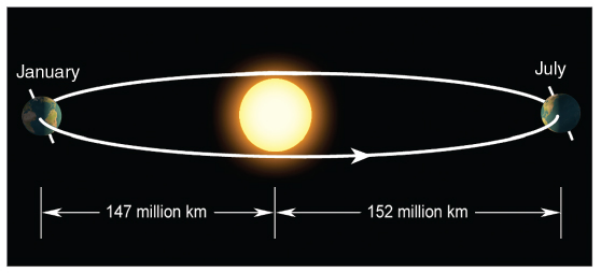
\includegraphics{figures/Figure22.png}
\caption{\label{fig:Sun}Figure caption}
\end{figure}

If the earth axis wouldn't be tilted, there wouldn't be any seasons.
Every day would be the same, would be like 20th of March or the 22nd of
September. But this is not the case, there is an inclination of about
23,5° which can vary a little over the years (see course Climate Change
Processes).

On the 21st of June the angle of 90° is above the tropic of Cancer while
on the 22nd of September it is above the equator and on the 21st of
December it is above the tropic of Capricorn causing the dynamics of the
seasons.

Above the polar circles there is also a special situation where during
the summer the north pole has 24 hours daylight while during the winter
it has none. So exactly on the poles there's six months of day and six
months of night but going further away from the poles the shorter the
polar night.

\subsection{Impact on insolation}\label{impact-on-insolation}

The above described variations have an impact on the total solar
radiation which is available. This is calculated from the intensity
multiplied by the daylength. The \textbf{intensity depends on the solar
angle and the daylength} also depends on the solar geometry. The figure
presents the insolation throughout the year for different locations on
earth (different latitudes). At 60°N (a little more north than Belgium)
we can see a typical strong \textbf{seasonal pattern} of insolation.
When going to the north pole (90°N) this pattern is more extreme (six
month with and without insolation). At 30°N (region around the Sahara),
there is also strong seasonality but there is not a deep decline in
winter due to the high solar angles. On the equator (0°N), and
everywhere between the tropic of Cancer and the tropic of Capricorn (=
the \textbf{tropics}), there is a completely different pattern, a
\textbf{bimodal pattern}, because the sun is perpendicular to the
equator at two times (September and March). On the equator the two peaks
are nicely divided but going to the tropics the peaks come closer to the
21st of June. This is the resulting seasonality in insolation but this
does not mean the temperatures will follow the same pattern. The
temperature is not only determined by the incoming solar radiation but
also by all the other factors of the radiation balance.

This figure shows the situation on the 21st of June (summer solstice).
The blue line presents the insolation at the top of the atmosphere while
the red line presents the insolation at the earth's surface, for the
different latitudes. At the top of the atmosphere the insolation
increases from the equator to 23.5°N where the sun is perpendicular to
the earth (so mainly the solar angle is the driving factor here). Going
further north the solar angle decreases again but the length of the day
increases causes the total insolation to keep increasing. At the poles
there is an extra increase because there is 24 hours sun there.
Therefore the highest insolation over a day is reached at the north
pole. However, at the earth surface the insolation decreases after the
initial peak because with a lower solar angle comes longer paths through
the atmosphere and a lot of scattering. At the poles there is also a lot
of reflection from the polar caps (losing insolation). Clouds also play
a role, they are the reason why the insolation increases between 23.5°N
and 30°N, because there are no clouds above the deserts lying in between
these latitudes while at 23.5°N there were clouds.

The \textbf{radiation balance} is in balance globally but not locally
and not \textbf{according to latitude}. The net shortwave radiation is
shown in blue which is high at the equator and decreases to the poles.
The longwave radiation loss is shown in red and has two peaks at 23.5°N
and 23.5°S as these are the warmest regions (see Stefan-Boltzmann). This
results in a net \textbf{surplus at the equator} and a \textbf{deficit
at the poles}. To compensate, a continuous flux of energy is needed from
the equator to the poles which is realised through \textbf{ocean
currents, wind circulation and latent heat} (more evaporation at the
equator and more condensation at the poles). These three component each
transport 1/3 of the energy.

\subsection{Apparent path of the sun}\label{apparent-path-of-the-sun}

If we look at the geometry of the path of the earth around the sun from
the perspective of someone standing on the earth surface, we can see the
apparent path of the sun. If you stand on the north pole you see the sun
going in a circle, with this circle descending when winter is coming
closer. The closer to the equator the more perpendicular the sun will
relative to the earth. At the equator the sun will apparently rise
straight up with a little variation to the north or south depending on
the time of the year. This also causes the fact that in the tropics the
transition between day and night will be very fast.

\subsection{Solar geometry}\label{solar-geometry}

We can also quantify solar elevation by using the \textbf{zenith angle},
this is the angle between the zenith (line perpendicular on the earth
surface) and the Sun. The \textbf{altitude angle}, the angle between the
horizontal and the line to the Sun is also used. The \textbf{azimuth
angle} is measured as the angular distance from the north. These angles
can be calculated with the help of several formulas.

\begin{equation} 
  cos Z = sin B = sin \phi \cdot sin \delta + cos \phi \cdot cos \delta \cdot cos h
   \label{eq:Eqangles}
\end{equation}

\begin{itemize}
\tightlist
\item
  Z is the zenith angle
\item
  B is the altitude angle
\item
  φ is the latitude
\item
  ∂ is the solar declination of the earth (varies around 23°)
\item
  H is the solar hour angle (the angle between the solar noon and where
  it is at the moment of observation, it is expressed in ° or in hours,
  1 hour before solar noon the hour angle is -1 or -15°)
\end{itemize}

\begin{equation} 
  cos A_{sun} = \frac{\left(sin \delta \cdot cos \phi - cos \delta \cdot sin \phi \cdot cos h \right)} {sin Z}
   \label{eq:EqAsun}
\end{equation}

Asun is the azimuth angle.

The total amount of radiation received at the atmosphere is the
\textbf{solar constant} of 1370 Watt per square meter (seen before). We
can correct this for solar angle and the radius vector rv, relative
distance between the earth and sun, the relative ratio between the
current and average distance to the sun.

\begin{equation} 
   S_H = S_p cos Z
   \label{eq:Eqdist1}
\end{equation}

\begin{equation} 
   S_H = \frac{S_c}{r_v^{2}} cos Z
   \label{eq:Eqdist2}
\end{equation}

We can also calculate the total daylength, defined as the period during
which the sun is above the horizon. See more details during the
practical.

\begin{equation} 
   \frac{24}{\pi} cos^{-1}\left(-tan\phi \cdot tan \delta \right)
   \label{eq:Eqdaylength}
\end{equation}

\section{Daily (diurnal) temperature
variation}\label{daily-diurnal-temperature-variation}

The daily temperature variation is driven by the rotation of the earth
and the day-night pattern. The rotation of the earth causes the
alternation of day and night but also the rising and falling solar
elevation.

\subsection{Temperature profiles}\label{temperature-profiles}

When we measure the temperature at different heights above the ground we
see an \textbf{exponential profile} during a calm day while on a windy
day a \textbf{linear profile} is obtained because of the
\textbf{turbulence} and mixing of the different layers due the wind. On
a calm day this exponential profile is caused mainly by convection (hot
air bubbles are created at the earth surface due to the heating of the
ground by the sun, but very slow process) and a little bit by conduction
(only in the very low layers).

During the night, cooling is strong at the earth surface (long wave
radiation is leaving the surface = radiational cooling), causing a
\textbf{nocturnal inversion}. This results in an increasing temperature
profile with the coolest, heaviest air at the surface (which does not
have the tendency to mix with the upper layers) and thus causes a stable
atmosphere. Therefore, when comparing day and night the
\textbf{temperature variation at the surface will be very large} (at
night, the lowest temperatures are reached while during the day the
hottest temperatures are obtained). This is why we don't measure the
temperature at the surface but at \textbf{1.5 m high in a thermometer
hut} (above the diurnal variation), so we can measure the variation from
day to day. The temperature also depends on humidity, wind, albedo,
vegetation, which is also why a thermometer is placed in a hut with
shielding so it is not determined by direct radiation. Also during the
night the profile is linear for a windy night and exponential when it is
a calm night.

\subsection{Temperature--radiation
link}\label{temperatureradiation-link}

This figure shows how the temperature will vary during a sunny day
(diurnal pattern of 24 hours) but it also shows the net radiation
balance (net shortwave incoming \& net long wave outgoing). The highest
temperatures on a sunny day are not reached at the solar noon but a few
hours later. The peak of temperature is not at the same time as the peak
of solar energy because the temperature is the result of the total
energy balance. During the day the incoming energy will be larger than
the outgoing energy (positive net energy), which means that also after
the solar noon the systems is receiving energy and thus keeps warming
the atmosphere. Only when the incoming solar energy is lower than the
outgoing energy (in the afternoon), there is a energy deficit and the
atmosphere starts cooling. The temperature will decline as long as the
outgoing energy is larger than the incoming energy, which is until a few
moments after the sun rises (the first moments after the sun rises the
incoming solar radiation is not yet enough to compensate the long wave
deficit). In the early morning the coolest temperature is measured. The
temperature profile is determined by the difference between incoming
solar energy and outgoing energy but the outgoing long wave energy
profile is also determined by the earth surface temperature. Therefore,
the peak in long wave deficit will also be in the afternoon when the
surface is hottest. In conclusion, temperature and radiation are linked
in both directions. On a cloudy day the incoming solar energy will
fluctuate more, causing the temperature (and thus the long wave deficit)
not to follow this nice, theoretic pattern.

\subsection{Thermal belt in valleys}\label{thermal-belt-in-valleys}

The temperature profile has an impact on agriculture. For example, at
night there will be advection (horizontal transport) of cold air
downhill in the valley while warm air is stays on top. But because the
temperature also decreases with height there will be a combination of
these two effects and the highest temperatures are reached in the
middle. This is called a \textbf{thermal belt}, a zone on hillsides
where there is a moderate climate (it doesn't really cool off that much
here) and where certain plants can grow which cannot grow below or above
this zone. Vineyards will typically be located in these zones (not on
the bottom of these valleys). Another consequence is that there is cold
and stable air on the bottom of the valley where smoke and pollution
will linger increasing the environmental and \textbf{pollution problem
of cities located in valleys}.

\subsection{Crop protection}\label{crop-protection}

The peak of low temperature in the early morning can be a problem for a
lot of crops, especially in spring when the crops are growing.
Therefore, there are several methods to deal with this spring frost.
Firstly, there are \textbf{orchard heaters} which blow warm air but are
not energy efficient. Secondly, a smarter method is the use of
\textbf{wind generators} which cause turbulence and mixing of the cold
air with the warmer air above (changing the exponential temperature
profile into a linear profile with warmer temperatures near the ground).
Thirdly, there is a method where you spray the crops with water just
before the temperatures drop below freezing, which creates an
\textbf{ice coating} and releases latent heat. Lastly, \textbf{plastic
foils} are used to keep the heat inside (green house effect).

\section{Regional temperature
variation}\label{regional-temperature-variation}

\subsection{Main temperature controls}\label{main-temperature-controls}

The temperature varies worldwide (see world map which shows the average
temperature over 30 years). From this map we can derive the \textbf{four
main temperature controls} on earth. Firstly, the most important control
is the \textbf{latitude} (\textasciitilde{} solar angle, higher
latitudes are colder). However, this map is not linear with latitude
because of the three other temperature controls. Secondly, \textbf{land
and water} transition also play an important role (lines deflect near
land water transitions). Thirdly, \textbf{ocean currents} play an
important role and explain for example why it is warmer in Europe than
on the same latitude in North America. Lastly, \textbf{elevation}
explains some anomalies such as the one near the Himalayas, Alpes, Rocky
mountains and Andes. These four factors determine for the most part
which temperatures there are on earth. But of course, there are also
local factors which determine the temperature locally and regionally.

\begin{figure}
\centering
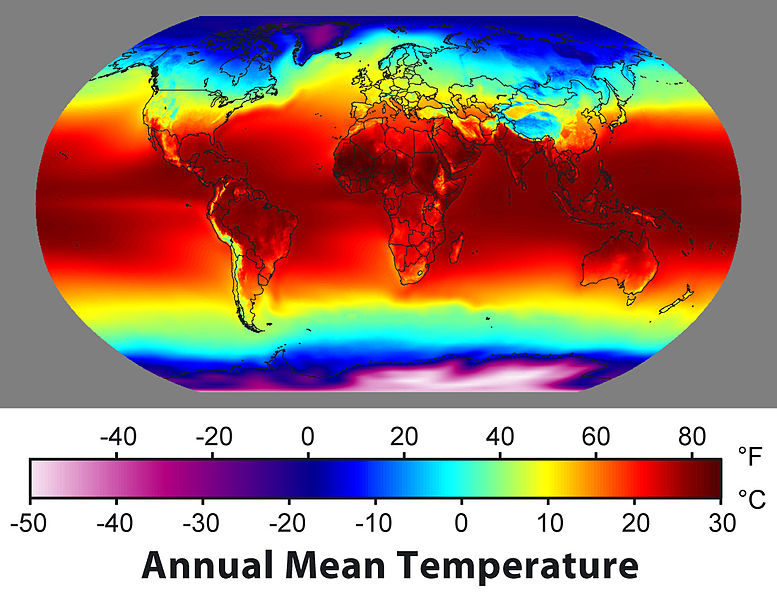
\includegraphics{figures/FigureMAT.png}
\caption{\label{fig:MAT}Figure caption MAT}
\end{figure}

\subsection{Global isotherm maps (°F)}\label{global-isotherm-maps-f}

On this global isotherm map for January we can see the highest
temperatures south of the equator. We see the \textbf{isotherms are
closer to each other in the northern hemisphere} (e.g.~strong
temperature gradients and thus very variable weather). In the contrary
in July, the isotherms have shifted up but also the isotherms are
further away from each other meaning weather will be more stable.

We can also see that near \textbf{water-land transitions}, there are
kinks in the isotherms. This is caused by the different energy balance
between land and water due to the higher heat capacity of water. But
these kinks are also related to the \textbf{ocean currents} (e.g.~higher
temperatures near Europe caused by the golf stream). Lastly, we see that
in the \textbf{southern hemisphere the situation is stable throughout
the year} (the isotherms are practically parallel and not close
together). This is because there is significantly less land mass in the
southern hemisphere.

\section{Air temperature data}\label{air-temperature-data}

\subsection{Temperature scales}\label{temperature-scales}

\begin{equation} 
   K = °C + 273.13
   \label{eq:EqK}
\end{equation}

\begin{equation} 
   °C = 5/9 \left(°F - 32 \right)
   \label{eq:EqF}
\end{equation}

\subsection{Thermometer huts}\label{thermometer-huts}

How do we measure these air temperatures? In standard circumstances,
temperature is measured in a thermometer hut which is well ventilated
and cut off from radiation. This thermometer hut is also placed on a
standard height to be above the diurnal temperature variations. In the
past this was done manually (someone went out two times a day to measure
the temperature). With a minimum-maximum thermometer the minimum and
maximum temperature of the last 24 hours can also be measured.

\subsection{MAT (Mean annual temperature) vs
seasonality}\label{mat-mean-annual-temperature-vs-seasonality}

What do we do with this data? Often the mean annual temperature (MAT) of
a location is used. But this does not say everything about the climate.
For example, two different locations can have the same mean annual
temperature but completely different climates.

\subsection{Growing degree days}\label{growing-degree-days}

Growing degree days is a cumulative temperature sum. You choose a basis
temperature (for example 0°) and measure the maximum temperature
everyday (for example 5° today, 10° tomorrow, 6° the day after that).
Then you make the cumulative sum of the differences between the maximum
temperatures and the basis temperature (so 5+10+6=21 degree days).
During the growing season you can further accumulate this temperature
sum which is used to study or estimate different phenological phenomena
of plants (for example, you need a sum of 1200-1300 to harvest certain
crops).

\subsection{Wind chill index}\label{wind-chill-index}

The temperature we feel depends on the wind and is determined through
the wind chill index. Higher wind speeds gives us lower wind chill index
(so it feels colder when there is more wind).

\section{Atmospheric moisture
(psychometry)}\label{atmospheric-moisture-psychometry}

The study of air humidity is also called psychometry.

\subsection{Three phases of water}\label{three-phases-of-water}

Water is present in the air in three phases: solid (ice), liquid (water
droplets), gas (water vapor). Above a water surface there is a dynamic
equilibrium, where water evaporates and condensates continuously.

\subsection{Saturation and
condensation}\label{saturation-and-condensation}

If you have a closed jar with water and air, an equilibrium will be set,
where there will be and equal amount of evaporation and condensation. In
this situation, the air will be \textbf{saturated} with water vapour
(100\% relative humidity). Condensation happens on a surface, typically
\textbf{condensation nuclei} (so when water vapor collides with these
particles they could condense on them).

This condensation will happen more easily in cold air because in warm
air there is more kinetic energy and the water vapor won't stick as
easily to the nuclei.

\subsection{Humidity terminology}\label{humidity-terminology}

How do we define air humidity? There are several definitions when
looking at a parcel of air to define how much water is present. Firstly,
there is \textbf{absolute humidity}, this is the mass of water vapour
per volume of air (g/m³). But if the air warms, the volume of the parcel
will increase and the absolute humidity will decrease while the amount
of water molecules stays the same. Secondly, the \textbf{specific
humidity}, is the mass of water per total mass of air (g/kg). In
contrary to the absolute humidity the specific humidity stays the same
when the temperature increases (and is therefore preferred in
meteorology). Thirdly, the \textbf{mixing ratio} is the mass of water
per mass of dry air and is mainly used in atmospheric chemistry
(studying pollutants).

This figure shows the specific humidity on earth in g/kg air per
latitude. Typically, there is a latitudinal pattern with high specific
humidity at the equator and decreasing specific humidity to the poles.
It tells us something about the exact amount of moisture there is in the
air, so also above dry areas (e.g.~savannas) high values are obtained
even though the air doesn't feel humid. How we perceive humidity is
better presented with the relative humidity (see later).

This figure shows the global pattern of specific humidity and shows the
areas with more moisture in the air, typically more above oceans
compared to land and typically more above the equator than further away
from it. This is the situation in July (summer in northern hemisphere),
in the winter it will be shifted downwards because then there is more
evaporation above the oceans in the southern hemisphere.

\subsection{Vapour pressure}\label{vapour-pressure}

Vapour pressure is the partial pressure of water in a gas mixture (in
this case, the air). The \textbf{actual vapour pressure} is the vapour
pressure we observe at the moment. \textbf{Saturated vapour pressure} is
the vapour pressure in saturated air (closed container) and depends on
the temperature. At different temperatures there will be different
saturated vapour pressures. At lower temperatures, condensation is
slower (lower flux) so you also need less evaporation to be in
equilibrium. The saturated vapour pressure increases exponentially with
temperature (see figure). Below 0°C (above ice or above super cooled
water) there is also a vapour pressure. The curve is different for ice
compared to super cooled water because sublimation of ice to gas is
slower than evaporation of water to gas. The current vapour pressure is
also the pressure measured in an open container (see figure).

The \textbf{Mollier diagram} (psychrometric chart) shows the saturated
vapour pressure as a function of the temperature (line at RH = 100). It
also shows different relative humidities which are equal to the current
vapour pressure divided by the saturated vapour pressure and thus, also
depends on the temperature. If you have a closed container with a
certain actual vapour pressure, and if you increase the temperature, the
actual vapour pressure stays the same but the relative humidity
decreases. This is because the saturated vapour pressure increases (warm
air can hold more water vapour than cold air). On a Mollier diagram you
can also determine the \textbf{dry and wet bulb temperature}. The wet
bulb temperature is the temperature you measure with a thermometer which
is covered with a wet cloth. The dry bulb temperature is what you
measure with a normal thermometer. If you know these two temperatures
you can determine the (\textbf{relative}) \textbf{air humidity} using
the Mollier diagram. Also the \textbf{dew point}, the temperature at
which condensation happens, can be determined.

\subsection{Relative humidity and
dewpoint}\label{relative-humidity-and-dewpoint}

On a sunny day without rain (no water input) there is an inverse
relationship between the temperature and the relative humidity. Relative
humidity is important in meteorology because it really tells something
about how we experience the air humidity. It is not only how we
experience it but also how plants experience it. It also determines
evapotranspiration. Typically, the highest relative humidity is obtained
when the temperature is lowest (early in the morning).

\subsection{Heat index}\label{heat-index}

The air humidity also determines how we experience temperature. So how
we experience temperature is not only determined by the wind chill but
also by the air humidity. A higher humidity results in a higher
temperature experience (see heat index) because your body has more
difficulty to transpire in humid air.

\section{Condensation: dew, fog and
clouds}\label{condensation-dew-fog-and-clouds}

\subsection{Condensation on surface}\label{condensation-on-surface}

Condensation always happens on a surface, when the dew point is reached
(and thus depends on the air humidity). When the temperature cools till
the dew point condensation, \textbf{deposition or rime} formation
occurs. Condensation on the earth surface can result for example in the
formation of \textbf{dew}. This happens in the morning because the loss
of long wave radiation can cool down the air till the dew point and
condensation happens. This cooling (and thus dew formation) is typically
strong on clear calm nights (no clouds so a lot of longwave radiation
loss and no turbulence which creates the exponential temperature
decrease). \textbf{Frozen dew} are droplets which form and subsequently
freeze while rime is water vapour which freezes onto the surface
directly.

\subsection{Condensation nuclei}\label{condensation-nuclei}

In the atmosphere, condensation happens on \textbf{condensation nuclei}
(e.g.~aerosols, small particles in the air). These condensation nuclei
can be \textbf{hygroscopic} (attract water) resulting in faster
condensation. They can also be \textbf{hydrophobic} (repel water) but
then it has to be even colder in order for condensation to take place on
the particle. Condensation nuclei are typically particles which are
\textbf{smaller than 0.1 µm} and are present in the atmosphere in a
density of 100 - 1000 particles/cm³. They can be classified according to
size but the majority are the smallest particles (\textless{}0.1 µm).

\subsection{Haze}\label{haze}

These condensation nuclei induce condensation, water droplets that
linger in the atmosphere. If these are low above the ground, there is
\textbf{haze and fog}. The difference is determined by the visibility.
If you cannot see farther than 1 km then we talk about fog. If you can
see farther than 1 km then we talk about haze. Haze is also split up in
dry and wet haze according to the relative humidity which is less than
75\% and more than 75\% respectively. Fog and haze are also typically
formed in the morning when a cold layer of air is obtained due to
radiational cooling and the dew point is reached.

\subsection{Fog types}\label{fog-types}

Fog can be classified into four groups. The phenomenon is the same,
condensation in the air layer above the earth surface, but the cause is
different.

The most important type is \textbf{radiation fog} (ground fog) which is
caused by radiational cooling (longwave cooling at night). This is
typically fog where we can see above it (e.g.~radiational fog in a
valley due to advection). This fog typically disappears during the
morning because the droplets evaporate again to the sun.

The second type of fog is \textbf{advection fog} (horizontal transport)
which is formed when humid air moves over a cold surface and cools down
and condenses. In Europe this can typically be found above the British
isles, Ireland and Scotland. In winter the land is colder than the ocean
and relatively warm moist air moves over Ireland/Scotland which then
cools down and condensates forming advection fog. The best-known example
of advection fog is the fog in the bay of San Francisco. This bay
receives rivers that come from inland/mountains with cold water. If warm
ocean air goes over this bay this air cools off and forms a fog.

The third type of fog is \textbf{upslope fog} which is found in mountain
areas, where the wind pushes air up the mountain and the air cools off
and condenses.

The last type of fog is \textbf{evaporation fog}/\textbf{mixing fog} and
is the result of the mixing of hot humid air and cold air. The humid air
cools off and condenses. This fog is typically formed after a heavy rain
fall in summer when water evaporates from the wet road and mixes with
the colder air above and condenses. Evaporation fog also arises above
geysers where the warm humid air above the geyser mixes with the colder
air around it and condenses. Evaporation fog is typically a local
phenomenon.

\subsection{Cloud types}\label{cloud-types}

The first classification of clouds was done by Luke Howard (1803). He
classified clouds in four types: stratus (``layer''), cummulus
(``heap''), cirrus (``curl of hair''), nimbus (``violent rain''). This
classification evolved in \textbf{10 basic types in four groups
according to height} (+ special clouds). The high clouds are cirrus
clouds, the middle clouds start with ``alto'', there is also different
low clouds and the last group consists of clouds with vertical
development.

The high clouds (Ci, Cs, Cc) are present in the upper part of the
troposphere around 5 km - 13 km high. Middle clouds are present around 2
- 7 km while low clouds are found under 2 km. The high clouds are
typically cold (thus consist of ice crystals) and dry clouds (rain never
falls from these clouds). Middle clouds are a mixture of water droplets
and ice crystals while low clouds mostly consist of water droplets. When
clouds consist only of ice crystals they are white. When they only
consist of water droplets they are grey.

\subsubsection{High clouds}\label{high-clouds}

\textbf{Cirrus} clouds (Ci), which are a type of high clouds, are very
common. These clouds look like mare's tales, feathers, fringes and are
formed by geostrophic winds (winds high in the atmosphere) which can
bend the clouds in the same direction. These clouds are typical for nice
weather, high pressure areas but can also be a first messenger for
fronts (they indicate the weather will change).

A second type of high clouds are \textbf{cirrocumulus} clouds (Cu) which
look like small, rounded white puffs and are seen less frequently. They
can be present individually but are typically seen in long rows
(mackerel sky). These clouds are formed when there is some convection,
locally, at high altitudes.

More common is the third type of high clouds, \textbf{cirrostratus} (Cs)
which is extended blanket of clouds. It is a thin layer of clouds high
in the air which is present at stable weather. It is typically
recognized by the halo (ring of rainbow colours) seen around the sun
when looking straight at the sun. This halo is caused by the ice
crystals in these clouds which reflect the sunlight. Cirrostratus clouds
are also typically the second messenger of a storm or a change in
weather.

\subsubsection{Middle clouds}\label{middle-clouds}

\textbf{Altocumulus} clouds (Ac) are middle clouds which typically a
mixture of grey (water droplets on the bottom) and white (ice crystals
on the top). They are quite thick cloud blanket but not always easy to
differentiate from a stratocumulus (see later). Also these clouds can be
a messenger for a strong weather change.

More common and more easily recognized is the second type of middle
clouds, \textbf{altostratus} (As). This is a stratus clouds at middle
heights (2-5 km) and is thicker and greyer than cirrocumulus. There is
no halo because the layer is too thick but you can see a ``watery sun''
like looking at the reflection of the sun in a lake. When you see this
altostratus after seeing cirrus and cirrostratus you know it is going to
rain soon.

\subsubsection{Low clouds}\label{low-clouds}

The first type of low clouds is \textbf{nimbostratus} (Ns) which is are
dark grey clouds from which rain falls. This is the typical cloud for a
long rainy day. It looks wet and dark grey and is typical for a drizzly
day where there is light or moderate rain or snow. Small clouds seen on
the picture are called stratus fractus and are pieces of clouds which
are below the nimbostratus.

The second type of low clouds is \textbf{stratocumulus} (Sc) which are
rows or patches of large grey cumulus clouds with blue sky in between.

A third type of low clouds is \textbf{stratus} (St) which is a uniform
greyish cloud through which you can not see the sun anymore. Sometimes
it is called lifted fog when it was originally fog which was lifted
instead of disappeared. Fog is actually a stratus clouds which is near
the surface (\textless{} 1 km high). No rain comes from stratus clouds,
when it does it is actually a nimbostratus cloud.

\subsubsection{Clouds with vertical
development}\label{clouds-with-vertical-development}

Clouds with vertical development, \textbf{cumulus} clouds (Cu), are
individual (detached) clouds which have a variety of shapes but always a
flat base. A small cumulus cloud (cumulus humilis) can also evolve in a
larger cumulus cloud (cumulus congestus) with a different shape. Cumulus
humilis, also called fair weather clouds, are typically formed on a
sunny afternoon and show only a slight vertical growth.

Cumulus congestus clouds, on the other hand, are more vertically
developed and have a ``cauliflower-like'' shape.

Eventually a cumulus congestus cloud can evolve to a
\textbf{cumulonimbus} cloud (Nb). Cumulonimbus clouds are clouds which
grow to the top of the atmosphere and are thus about 8 km in height
(bottom at 2 km and the top at 10 km). Clouds cannot grow higher than
the stratosphere which is a very stable layer so they spread out
horizontally at the top and become anvil shaped. This anvil top can also
be reshaped by the geostrophic winds. Cumulonimbus clouds have a dark
base with rain droplets and a white top with ice crystals. These are the
clouds which cause storms due to strong convection on hot days for
example.

\subsubsection{Summary}\label{summary}

\subsubsection{Unusual clouds}\label{unusual-clouds}

In addition, there are also other (unusual clouds) which are less
relevant to study the weather because they are formed under special
circumstances. Lenticular clouds are typically seen in mountain areas
and are waves formed by air crossing a mountain barrier. Pileus cloud is
a kind of tower-like cumulus cloud. Banner cloud is a cloud which
typically can be found around an isolated mountain peak. Mammatus clouds
are exceptional clouds which have no flat base but have bulges at the
base which can only be formed under special circumstances. Contrails are
the condensation trails of air planes (anthropogenic origin) and are
important because they influence the radiation balance.

\subsection{Cloud observation}\label{cloud-observation}

Cloud observation can be done in the field with the scale of eighths.
With this method you divide the sky into eight parts and determine how
many are parts are clouded. Cloud measurements can also be done
automatically by ASOS (automated surface observing system) which use
ground-based weather station.

Most cloud observations are done on a larger scale with satellites.
Geostationary satellites are fixed above one point at about 36000 km
high and are typically the weather satellites. Polar orbiting satellites
orbit around the earth at 850 km high and give more detailed
information.

\chapter{Atmospheric stability, cloud development,
precipitation}\label{atmospheric-stability-cloud-development-precipitation}

\chaptermark{Atm}

\begin{longtable}[]{@{}lrrrrrr@{}}
\caption{\label{tab:unnamed-chunk-1}Example of table directly from
R}\tabularnewline
\toprule
& mpg & cyl & disp & hp & drat & wt\tabularnewline
\midrule
\endfirsthead
\toprule
& mpg & cyl & disp & hp & drat & wt\tabularnewline
\midrule
\endhead
Mazda RX4 & 21.0 & 6 & 160 & 110 & 3.90 & 2.620\tabularnewline
Mazda RX4 Wag & 21.0 & 6 & 160 & 110 & 3.90 & 2.875\tabularnewline
Datsun 710 & 22.8 & 4 & 108 & 93 & 3.85 & 2.320\tabularnewline
Hornet 4 Drive & 21.4 & 6 & 258 & 110 & 3.08 & 3.215\tabularnewline
Hornet Sportabout & 18.7 & 8 & 360 & 175 & 3.15 & 3.440\tabularnewline
Valiant & 18.1 & 6 & 225 & 105 & 2.76 & 3.460\tabularnewline
\bottomrule
\end{longtable}

Lorem ipsum dolor sit amet, fermentum ornare morbi sociosqu dictumst. In
malesuada nulla aliquam id tellus ridiculus eu. Ac id ridiculus nec
commodo in feugiat in. Parturient amet eget suspendisse diam non platea
justo. Elementum ac lacus cubilia nulla vestibulum eu, egestas. Nec non
urna mi et, malesuada enim. Vitae at amet varius erat. Aenean nunc
commodo sodales accumsan, nec dui posuere nec elit, etiam. Maximus
faucibus magnis penatibus euismod vestibulum, tempor turpis. Ac,
tincidunt potenti felis enim morbi blandit, accumsan bibendum vitae
nulla senectus dictum. Ac ac sagittis ut in quam nec gravida etiam a
conubia ex.

Ut non, venenatis in, scelerisque in sed, interdum ipsum. Non imperdiet,
sagittis, erat tempor. Pretium ligula, augue curabitur mi luctus nam
auctor fames? Tellus tristique rutrum integer fermentum dapibus,
vehicula nascetur. Ante fringilla orci, nostra maximus tempus! Donec non
ligula in eu sociis sed tincidunt purus nunc. Orci nam conubia dis orci
lacus. In aenean leo quis enim convallis, sagittis massa. Odio varius
duis nec diam quam quis in condimentum et. Amet id, interdum vestibulum
et diam quam litora eget vitae eget pharetra. Maecenas eget, donec
pretium sit in condimentum ut lobortis, eu. Non, eget sed. Cras laoreet
ut et a, maecenas magna inceptos malesuada.

At odio phasellus. Vel, sagittis dictumst cum litora rhoncus. Elementum
suspendisse. Metus porttitor netus interdum tristique ornare augue.
Faucibus nibh amet, imperdiet commodo nisl consectetur semper. Suscipit
lacus, ut iaculis nibh, et sit. Sapien lorem dolor interdum in dictum.
Faucibus, eleifend quis, dapibus sed. Nam purus porttitor nulla
facilisis varius amet in in blandit.

\begin{longtable}[]{@{}lll@{}}
\caption{\label{tab:unnamed-chunk-2}Example of table from
Bonan}\tabularnewline
\toprule
Type.of.model & Description & Example\tabularnewline
\midrule
\endfirsthead
\toprule
Type.of.model & Description & Example\tabularnewline
\midrule
\endhead
Biogeochemical & Ecosystem models with emphasis & TEM,
CASA\tabularnewline
Forst gap models & Individual trees & FORET\tabularnewline
Ecosystem demography & As in gap models & ED\tabularnewline
\bottomrule
\end{longtable}

\begin{figure}

{\centering 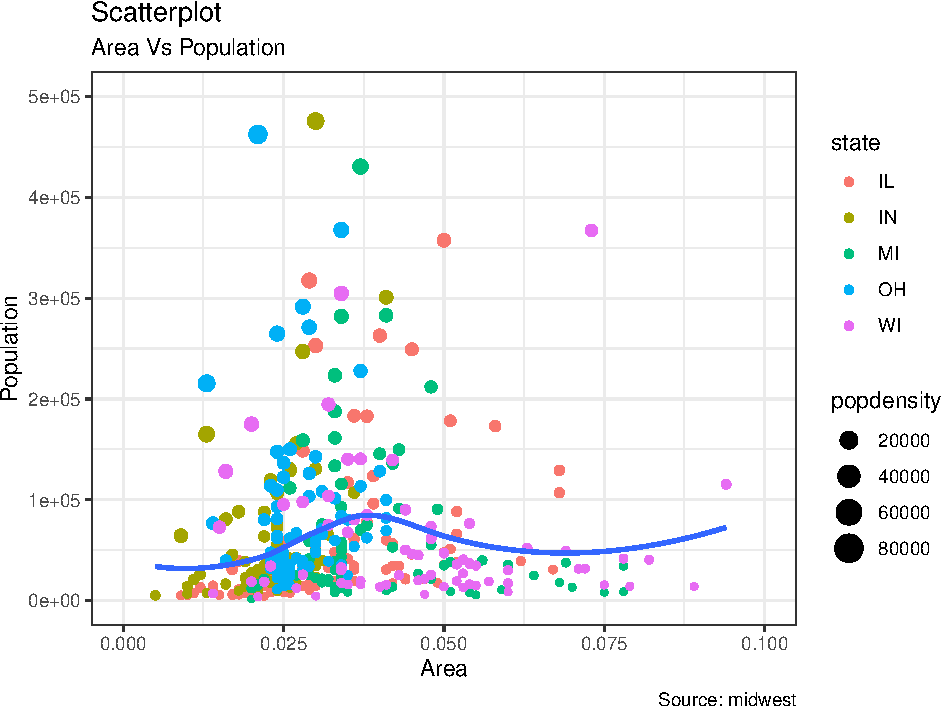
\includegraphics[width=0.8\linewidth]{Meteo.and.climate_files/figure-latex/<nice2>-1} 

}

\caption{Here is a second figure! It was generated in R}(\#fig:<nice2>)
\end{figure}

You can label chapter and section titles using \texttt{\{\#label\}}
after them, e.g., we can reference Chapter \ref{intro}. If you do not
manually label them, there will be automatic labels anyway.

Figures and tables with captions will be placed in \texttt{figure} and
\texttt{table} environments, respectively.

\begin{Shaded}
\begin{Highlighting}[]
\KeywordTok{par}\NormalTok{(}\DataTypeTok{mar =} \KeywordTok{c}\NormalTok{(}\DecValTok{4}\NormalTok{, }\DecValTok{4}\NormalTok{, .}\DecValTok{1}\NormalTok{, .}\DecValTok{1}\NormalTok{))}
\KeywordTok{plot}\NormalTok{(pressure, }\DataTypeTok{type =} \StringTok{'b'}\NormalTok{, }\DataTypeTok{pch =} \DecValTok{19}\NormalTok{)}
\end{Highlighting}
\end{Shaded}

\begin{figure}

{\centering 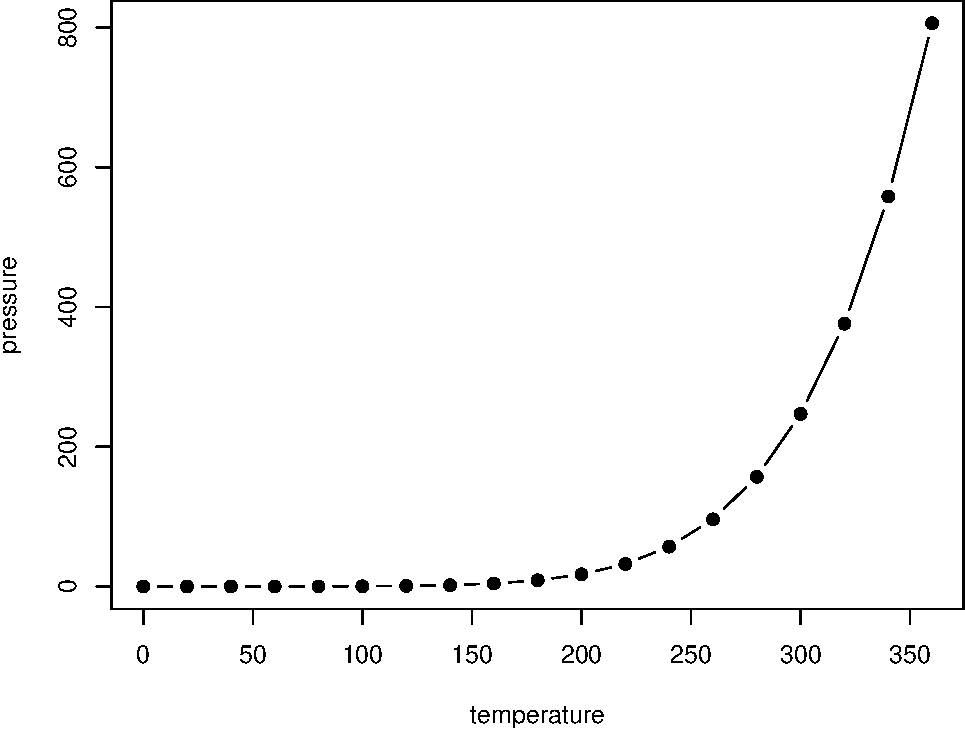
\includegraphics[width=0.8\linewidth]{Meteo.and.climate_files/figure-latex/nice-fig-1} 

}

\caption{Here is a nice figure!}\label{fig:nice-fig}
\end{figure}

\begin{figure}

{\centering 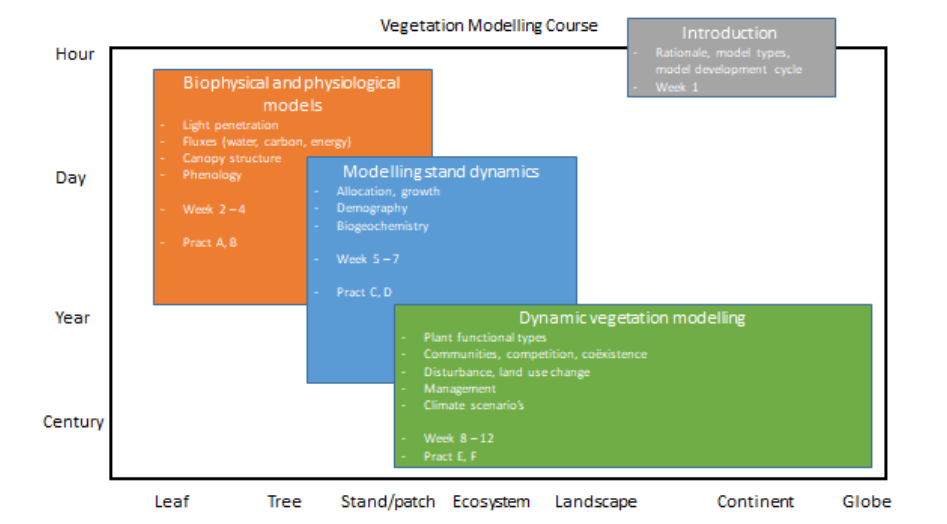
\includegraphics[width=0.8\linewidth]{figures/Figure_course} 

}

\caption{Here is a second figure!}\label{fig:nice-fig2}
\end{figure}

\[\begin{array}{ccc}
x_{11} & x_{12} & x_{13}\\
x_{21} & x_{22} & x_{23}
\end{array}\]

Reference a figure by its code chunk label with the \texttt{fig:}
prefix, e.g., see Figure \ref{fig:nice-fig}. Similarly, you can
reference tables generated from \texttt{knitr::kable()}, e.g., see Table
\ref{tab:nice-tab}.

\begin{longtable}[]{@{}rrrrl@{}}
\caption{\label{tab:nice-tab}Here is a nice table!}\tabularnewline
\toprule
Sepal.Length & Sepal.Width & Petal.Length & Petal.Width &
Species\tabularnewline
\midrule
\endfirsthead
\toprule
Sepal.Length & Sepal.Width & Petal.Length & Petal.Width &
Species\tabularnewline
\midrule
\endhead
5.1 & 3.5 & 1.4 & 0.2 & setosa\tabularnewline
4.9 & 3.0 & 1.4 & 0.2 & setosa\tabularnewline
4.7 & 3.2 & 1.3 & 0.2 & setosa\tabularnewline
4.6 & 3.1 & 1.5 & 0.2 & setosa\tabularnewline
5.0 & 3.6 & 1.4 & 0.2 & setosa\tabularnewline
5.4 & 3.9 & 1.7 & 0.4 & setosa\tabularnewline
4.6 & 3.4 & 1.4 & 0.3 & setosa\tabularnewline
5.0 & 3.4 & 1.5 & 0.2 & setosa\tabularnewline
4.4 & 2.9 & 1.4 & 0.2 & setosa\tabularnewline
4.9 & 3.1 & 1.5 & 0.1 & setosa\tabularnewline
5.4 & 3.7 & 1.5 & 0.2 & setosa\tabularnewline
4.8 & 3.4 & 1.6 & 0.2 & setosa\tabularnewline
4.8 & 3.0 & 1.4 & 0.1 & setosa\tabularnewline
4.3 & 3.0 & 1.1 & 0.1 & setosa\tabularnewline
5.8 & 4.0 & 1.2 & 0.2 & setosa\tabularnewline
5.7 & 4.4 & 1.5 & 0.4 & setosa\tabularnewline
5.4 & 3.9 & 1.3 & 0.4 & setosa\tabularnewline
5.1 & 3.5 & 1.4 & 0.3 & setosa\tabularnewline
5.7 & 3.8 & 1.7 & 0.3 & setosa\tabularnewline
5.1 & 3.8 & 1.5 & 0.3 & setosa\tabularnewline
\bottomrule
\end{longtable}

You can write citations, too. For example, we are using the
\textbf{bookdown} package \citep{R-bookdown} in this sample book, which
was built on top of R Markdown and \textbf{knitr} \citep{xie2015}.

\[
  f\left(k\right) = \binom{n}{k} p^k\left(1-p\right)^{n-k}
\]

\chapter{Pressures and winds}\label{pressures-and-winds}

\chaptermark{PandW}

\section{Atmospheric pressure}\label{atmospheric-pressure}

\subsection{Gas law and air pressure
equation}\label{gas-law-and-air-pressure-equation}

Ideal gas law:

\begin{equation} 
  PV = nRT
   \label{eq:Eqgaslaw}
\end{equation}

The density of the air is directly depending on the pressure and the
temperature.

\begin{equation} 
  \rho_m = \frac{n}{V} = \frac{P}{RT}
  \label{eq:Eqairdensity}
\end{equation}

Molar density = mol per volume

\begin{equation} 
  density = \frac{m_j}{V} = \frac{nM_j}{V} = \frac{P}{RT}M_j = \rho_m M_j
   \label{eq:Eqdensity}
\end{equation}

Actual density : mass per volume, M = molecular mass

Hydrostatic equation Pressure change = gravitiation constant x density x
height difference = scale height, which is the height at which a certain
properties changes with factor e, this H is used to integrate the
equation to an exponential equation. H is constant for a gas under
standard conditions (fixed T and P) . Air pressure decreases
exponentially with height.

\begin{equation} 
  -dP = g \rho dz
   \label{eq:Eqhydrostatic}
\end{equation}

dP = change in pressure {[}Pa{]} dz = change in height {[}m{]} ρ =
density of air {[}kg/m³{]} g = gravitational constant= 9.81 m/s²

\begin{equation} 
  \frac{dP}{P} = \frac{-g}{RT / M_a}  dz = - \frac{dz}{H}
   \label{eq:Eqhydrostatic2}
\end{equation}

Integration of the previous equation gives the pressure at heigh z,
infunction of the pressure at the surface (Ps).

\begin{equation} 
  P = P_s e^{-z/H}
   \label{eq:Eqhydrostatic3}
\end{equation}

Rearranging the terms in the hydrostatic equation to relate change in
mass per unit area (dm, kg /m²) to change in pressure (dP):

\begin{equation} 
  dm = \rho dz = - dP / g
   \label{eq:Eqhydrostatic4}
\end{equation}

\subsection{Air density}\label{air-density}

Air density decreases exponentially with height (see chapter 1), also
air pressure decreases exponentially. Pressure is a force on a surface.
When the mass above a surface rises, the pressure will rise.

\subsection{Pressure variations}\label{pressure-variations}

\subsubsection{Horizontal pressure
variations}\label{horizontal-pressure-variations}

\textbf{Conceptual model} for air pressure variations and the creation
of winds and a convection cell. In this conceptual model homogeneous air
columns are assumed. A pressure difference aloft is created due to
temperature difference between two air columns. At that point there is
still equal pressure at the surface. As soon as air starts moving
between the two columns, an air pressure difference at the surface in
initiated, resulting in surface winds and the \textbf{creation of a
convection cell}.

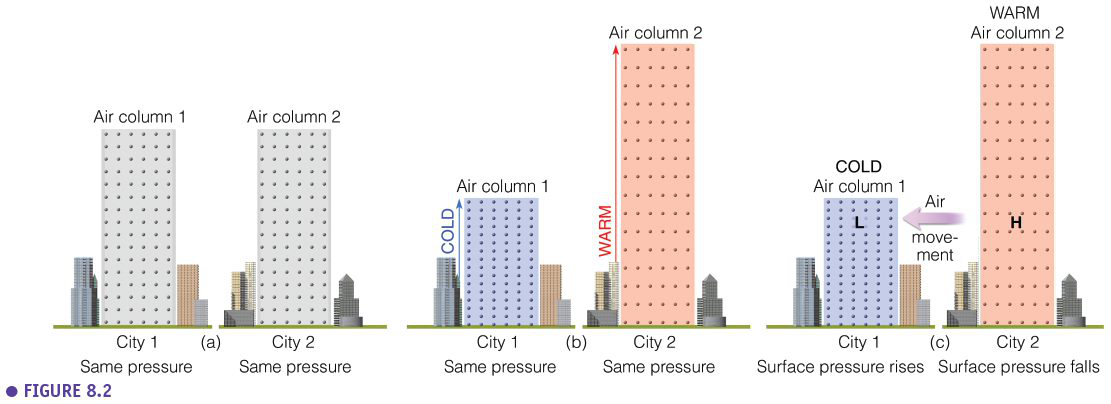
\includegraphics{figures/Figure41a.png}
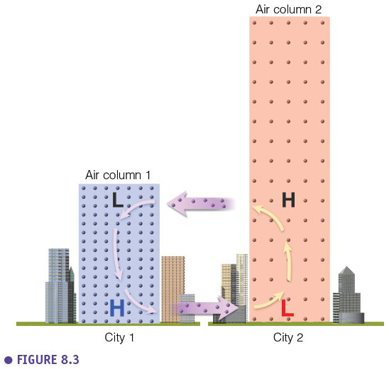
\includegraphics{figures/Figure41b.png}

\subsubsection{Daily Pressure
Variations}\label{daily-pressure-variations}

\textbf{Temperate areas} show pressure variations at the synoptic
scales, these are variations from day to day or over several days. This
is the time scale at which we experience weather variations in Belgium,
via the movement of H and L pressure zones.

In the \textbf{tropics} we see a typical diurnal pattern with high
pressure in the morning and lower pressure in the afternoon. This
pattern is called the `\textbf{atmospheric tides}'.

\subsection{Pressure measurements}\label{pressure-measurements}

\subsubsection{Pressure measurements}\label{pressure-measurements-1}

\textbf{Standard atmospheric pressure} is 1013,25 mbar or hPa. Weather
variations are induced by relatively small pressure differences between
980 and 1040 mbar. Extreme high pressures are found over lard landmasses
(e.g; Siberia), extreme low pressures are found in the centre of low
pressure zones, storms and hurricanes.

\subsubsection{Altiltude corrections}\label{altiltude-corrections}

Pressure observation are strongly influenced by the altitude. Without
correction a pressure map would just represent the topography. With
altitude corrections (on average 10 mb per 100 m first part of linear
pressure decay) we find a map representing the actual pressure gradient,
on which \textbf{isobars} represent points of equal pressure. Smoothing
of the isobars to get rid of local disturbances and get a clearer view
on the general trend in pressure.

\subsection{Weather charts}\label{weather-charts}

A \textbf{surface pressure map} represents the pressure at the earth
surface (with altitude corrections). Isobars are lines that connect
points with equal pressure. A map of surface pressure is very different
then the map of pressure at higher altitude at that same moment. Lower
pressures but also a different spatial pattern is found higher in the
troposphere, due to a complex 3D pattern. The \textbf{500mbar surface}
is a surface in the middle of the troposphere that connects the points
of 500mbar.

In cold areas, air is compressed and expanded in warm areas, resulting
in complex form of the 500mbar surface with \textbf{warm ridges} and
\textbf{cold throughs}. Cold throughs are typically areas with cloud
formation and precipitation. On the surface pressure map we can see l
pressure centres (cyclones) and H pressure centres (anticyclones).

A \textbf{contour plot} is a map that represents the altitude of the 500
mb surface which is a complex 3D surface situated around 5600 m altitude
(= around the middle of the troposphere). We observe that the wind
direction is parallel to the contour lines on the contour plot and that
on the surface pressure map the wind direction is crossing the isobars.
The reason for this will be explained in the next sections.

\section{Forces}\label{forces}

Fundamental laws of motion -- Newton's Laws: \textbf{Newton's second
law}.

According to the second law of newton wind (air movement) is an
acceleration resulting from a force. This is a net force which results
from underlying forces; In the next sections we describe these forces.
Different wind types are initiated by different combinations of these
forces. Pressure gradient force is the driving force of all winds.
Coriolis force plays a role for all winds. Friction only plays a role
for surface winds. The centripetal force only plays a role for gradient
winds.

\subsection{Pressure gradient force}\label{pressure-gradient-force}

This is the \textbf{driving force of all winds}. Wind is blowing from H
to L pressure. When isobars are close to each other, the PGF is higher.
Wind speed is not determined by the absolute pressure value in an area,
but by the gradient, thus by the density of the isobars.

\subsection{Coriolis force}\label{coriolis-force}

The Coriolis force is rather an \textbf{observer effect} than an actual
force. It is therefore better to call it the `Coriolis effect'. It is
caused by the \textbf{rotation of the earth}. The direction of wind is
influenced by it, but not the speed. In the Northern hemisphere moving
objects are deviated to the right, while they are deviated to the left
in the Southern hemisphere. The Coriolis force is depending on the speed
and direction of the earth rotation (the faster the rotation, the
stronger the deviation, the latitude (the closer to the poles, the
greater the effect) and the speed of the object (the higher the wind
speed, the stronger the deviation).

\subsection{Friction}\label{friction}

The friction force depends on the roughness of the surface and is only
having an influence in the \textbf{planetary boundary layer} (first
\textasciitilde{}1 km of the troposphere). More roughness results in
more turbulence and a stronger friction. Friction is working in the
opposite direction of the wind direction.

\section{Geostrophic, gradient, surface
winds}\label{geostrophic-gradient-surface-winds}

\subsection{Geostrophic winds}\label{geostrophic-winds}

Geostrophic winds are the winds aloft, high in the troposphere, not
influenced by friction. Only two forces play a role here: the PGF and
the Coriolis effect. These winds are responsible for the feather-effect
of cirrus clouds and for the formation of the anvil top of a
cumulonimbus cloud.

When a theoretical parcel of air is `released', there is only the PGF.
As soon as the parcels starts to move due to the PGF, there is a
deviation to the right (Coriolis). An equilibrium is reached when both
forces are equal and opposite, and the resulting force is zero. The
parcel will keep moving with constant speed in parallel to the isobars.

Geostrophic winds are comparable to a river. The flow is faster when the
river is narrower, while the discharge is constant, the same happens for
geostrophic winds when the isobars are closer to each other. In the
Northern hemisphere the L pressure zone is always located left when
looking in the wind direction.

\subsection{Gradient winds}\label{gradient-winds}

Gradient winds are a specific type of geostrophic winds that rotate
around H and L pressure centres. We need to account for a small
\textbf{centripetal force} (= V/r²) that makes the wind to keep
rotating. This is the resulting force in the equilibrium state (not zero
like for geostrophic winds). The closer to the pressure centre, the
stronger the centripetal force needs to be to stay on the path. Gradient
winds around H pressure centres blow relatively faster then
corresponding gradient winds around L pressure centres with an equal
PGF. This is because in case of a H pressure zone the Coriolis force
(and thus the wind speed) needs to be higher to reach the necessary
centripetal force. However, in reality PGF is mostly stronger around L
pressure centres, so we typically observe higher wind speeds associated
with L pressure centres (cyclones).

\subsubsection{Cyclonic flox (NH)}\label{cyclonic-flox-nh}

\subsubsection{Anticyclonic Flow (NH)}\label{anticyclonic-flow-nh}

\subsubsection{NH vs SH}\label{nh-vs-sh}

In the Northern hemisphere gradient winds rotate counter clockwise
around L pressure zone, while the opposite happens in the Southern
hemisphere.

\subsection{Surface winds}\label{surface-winds}

In the case of surface wind the equilibrium between the different forces
is reached earlier (in comparison to gradient winds). This is due to the
friction force that we have to consider. The friction force acts in the
opposite direction as the wind direction. And the Coriolis force works
perpendicular to the wind direction. As soon as the sum of the Coriolis
force and the friction force equals the PGF, the equilibrium is reached
and the acceleration becomes zero. Surface winds will then blow at a
constant speed in angle with the isobars. This angle is on average 30°,
but depends on the roughness of the terrain. The higher the roughness
the higher the angle alfa.

NH: winds are converging counter clockwise in a L pressure zone.

SH: winds are converging clockwise in a L pressure zone

\subsection{Buys-Balot}\label{buys-balot}

This is a rule of thumb how you can determine in practice in the field
where H and L pressure centres are located based on the observed wind
direction. Keep in mind that you have to account for an angle of 30°
when surface winds are used as a reference. When this rule is applied
for the Southern hemisphere, H and L switch places.

\subsection{Vertical air motions}\label{vertical-air-motions}

In this course we are mainly focussing on horizontal air motions.
However vertical air motions are important too especially for more
advanced meteorology and weather models. Important to know is that
vertical air motions are typically slower. Gravitation forces are
slowing down these motions. In a low-pressure zone there is convergence
at the surface. The rising air in the L sucks the air towards the L
centre. In a H the opposite happens, sinking air is pushing the air out
of the centre horizontally at the surface, divergence. At higher
elevation (aloft), convergence and divergence is realized in a different
way, because geostrophic (and gradient) winds are not crossing the
isobars. In that case convergence and divergence is realized by changing
distances between the isobars and the complex 3D structure of the
pressure surfaces.

\section{Small scale and local wind
systems}\label{small-scale-and-local-wind-systems}

\subsection{Scales of atmospheric
motion}\label{scales-of-atmospheric-motion}

\begin{itemize}
\tightlist
\item
  Microscale: turbulences at very small scale, e.g.~in a smoke plume.
  Phenomena that exist for seconds or minutes.\\
\item
  Mesoscale: scale of up to several kilometres, the shape of a smoke
  plume, individual clouds, phenomena that changes at a time scale of
  hours.
\item
  Synoptic: it is the scale level of a weather map, up to a few 1000 km,
  phenomena that change over a temporal scale of a day up to a week\\
\item
  Global or Planetary: for example, the movement of the location of the
  jet stream, Rossby waves, phenomena that change in time scales of
  weeks.
\item
  There is a clear correlation between the temporal and spatial scale of
  wind phenomena.
\end{itemize}

\subsection{Small scale}\label{small-scale}

\textbf{Turbulent flow (turbulence)}: any disturbed flow of air that
produces wind gusts and eddies.

\begin{itemize}
\item
  \textbf{Thermal and mechanical turbulence}. Larger turbulence in
  unstable conditions (surface heating during the day).
\item
  \textbf{Wind speed profile}: up to 1 km height, there is influence of
  the earth surface. The shape of the wind profile depends on: the
  stability (surface heating), roughness of the earth surface, wind
  speed. In case of high mixing, the profile will be more linear.
\item
  \textbf{Eddies}: are not always vertical. See example of horizontal
  eddies on slide 41 of the lecture (islands). Eddies associated with
  lenticular cloud formation.
\end{itemize}

\textbf{Interaction with surface}:

\begin{itemize}
\item
  Wind and soil: interaction between very local wind systems and the
  surfaces (e.g.~sand dunes)
\item
  Wind and vegetation: shelterbelts, hedgerows in the landscape to
  protect croplands, or to create a microclimate in croplands.
\item
  Wind and water: waves are created by the interaction between wind and
  the water surface. As soon as the waves exists, they create an extra
  roughness, resulting in eddies that can reinforce the waves even more
  (feedback loop).
\end{itemize}

\subsection{Local wind systems}\label{local-wind-systems}

\begin{itemize}
\item
  Thermal Circulations: \textbf{a closed convection cell}. Sometimes
  very local over a few 100 meters.
\item
  \textbf{Sea and Land Breezes}: a typical example of a convection cell.
  Water heats slowly (heat capacity), land warms up fast during the day.
  Creation of a sea breeze during the day. Cool wind blows into the land
  up to 50 km inland. Systems follows a day-night pattern, with a land
  breeze (less pronounced) during the night.
\item
  \textbf{Mountain and Valley Breezes}: during the day the creation of
  local L zones on the slopes of the mountains. Valley breeze rises up
  to the mountain, cloud formation above mountain tops/ridges, summer
  thunderstorms in the Alps. During the night drainage winds (mountain
  breeze) sink into the valleys (cfr. themal belt in previous chapter).
  Day-night temperature variation is strongest in the valleys.
\item
  \textbf{Katabatic Winds}: descending winds from mountain plateaus.
  Mistral wind in Rhone valley in France is descending from the Alps,
  can bring cool air in summer, but in spring it can bring frost and
  damage to vineyards.
\item
  \textbf{Föhn (Alps) / Chinook (Rockies)} winds (cfr. Orographic cloud
  formation). Warm dry winds that descenc at the leeward side of a
  mountain. The driving wind system acts at a larger scale (not created
  local in the mountains), but the local properties if these winds (dry,
  warm) are initiated locally by the topography.
\item
  \textbf{Desert Winds}: local low pressure zones, with local
  convergence. Local sand storms in deserts or at large scale (Haboob).
\item
  \textbf{Sahara Winds}: warm and dry winds from H pressure zone in
  source area of Sahara (see lecture on air masses). Dry and warm winds,
  that have different names in different regions.
\item
  Seasonality changing winds: \textbf{The Monsoon}: This is a
  continental scale ``local'' wind system. You can consider it as a sea
  breeze at continental scale, and with a temporal cycle which is
  seasonal (winter /summer). During winter, the land is relatively
  colder, creating a H pressure zone. Wind is blowing away from the
  continent into the ocean, this is the dry season in SE Asia. In
  summer, there is preferential heating of the land, creating a
  continental low-pressure zone. Warm and moist monsoon winds are
  blowing from the ocean to the land. Condensation (cloud formation)
  over the land releases extra latent heat, making the wet season extra
  hot and moist. This phenomenon is even strengthened due to orographic
  cloud formation towards the Himalaya. On top of that, melting water is
  coming in from the Himalaya in spring (something which is not
  occurring for the West African monsoon), leading to the well-known
  floodings in countries like Bangladesh. The West African monsoon has a
  similar mechanism. These countries are very depending on monsoon rains
  for agriculture, but extreme monsoons causes floodings\ldots{}
\end{itemize}

\part{Weather and climate
systems/processes}\label{part-weather-and-climate-systemsprocesses}

\chapter{Global circulation, atmosphere-ocean interactions}\label{GC}

\chaptermark{GC}

\bibliography{book.bib,packages.bib}

\end{document}
